\documentclass{beamer}
\usepackage[utf8]{inputenc}

\newcommand{\listingssize}{\normalsize}

%\newcommand{\titulek}{C\# - Úvod, datové typy, základní konstrukce}
\newcommand{\titulek}{C\# - Objektové typy}
\newcommand{\autor}{Ing. Roman Diviš}

\newcommand{\predmet}{\titulek}

\usepackage[czech]{babel} 
%\usepackage[IL2,T1,T2A]{fontenc} 
\usepackage[T1]{fontenc} 

%\usetheme{JuanLesPins}
\usetheme{Boadilla}

%%%%%%%%%%%%%%%%%%%%%%%%%%%%%%%%%%%%%%%%%%%%%%%%%%%
\setbeamertemplate{footline}[frame number]{}
\setbeamertemplate{navigation symbols}{}
\setbeamertemplate{blocks}[rounded][shadow=false]
%\setbeamertemplate{blocks}[default]
%\setbeamertemplate{background canvas}[vertical shading][bottom=white,top=structure.fg!5]

% zrušení mezer mezi bloky
\setlength{\medskipamount}{0pt}
\setlength{\smallskipamount}{0pt}

% pro vkládání obrázků
\usepackage{graphicx} 
% pro použití víceřádkových komentářů
\usepackage{verbatim} 
% H modifikátor figure
\usepackage{float}
% barvičky
\usepackage{xcolor,colortbl}
\usepackage{subfig}


\newcommand{\rc}{\cellcolor{red!25}}
\newcommand{\bc}{\cellcolor{blue!25}}
\newcommand{\gc}{\cellcolor{gray!25}}
\newcommand{\grc}{\cellcolor{green!25}}

\newcommand{\cpp}[1]{{\footnotesize$^{C++#1}$}}

\newcommand{\thisse}{\color{blue}\textbf{{\tiny this}}$\searrow$}
\newcommand{\thise}{\color{blue}\textbf{{\tiny this}}$\rightarrow$}

\usepackage{tikz}
\usetikzlibrary{arrows,shapes}
\newcommand{\tikzmark}[1]{\tikz[remember picture] \node[coordinate] (#1) {#1};}

% listingy
\usepackage{listings}

\newcommand{\commentcolor}{\color[rgb]{0.133,0.545,0.133}}
\lstset{
  tabsize=2,
  language=matlab,
  basicstyle=\small, %\listingssize,% \ttfamily,
  %upquote=true,
  mathescape=false,
  aboveskip=0pt, %{1.5\baselineskip},
  % zrušení nadbytečné mezery za posledním řádkem
  belowskip=0pt,
  columns=fullflexible,
  showstringspaces=false,,
  breaklines=true,
  prebreak = \raisebox{0ex}[0ex][0ex]{\ensuremath{\hookleftarrow}},
  frame=none,
  showtabs=false,
  showspaces=false,
  showstringspaces=false,
  identifierstyle=\ttfamily,
  keywordstyle=\color[rgb]{0,0,1}\bfseries,
  commentstyle=\color[rgb]{0.133,0.545,0.133},
  stringstyle=\color[rgb]{0.627,0.126,0.941},
  language=Java,
  inputencoding=utf8,
  extendedchars=true,
  literate={á}{{\'a}}1 {ã}{{\~a}}1 {é}{{\'e}}1 {ž}{{\v{z}}}1 {ý}{{\'y}}1 {ě}{{\v{e}}}1 {ř}{{\v{r}}}1 {í}{{\'i}}1 {ů}{{\r{u}}}1 {č}{{\v{c}}}1 {ú}{{\'u}}1 {š}{{\v{s}}}1 {ť}{{\v{t}}}1 {Č}{{\v{C}}}1 {Š}{{\v{S}}}1 {ň}{{\v{n}}}1 {Ř}{{\v{R}}}1 {ó}{{\'o}}1 {ď}{{\v{d}}}1 {ú}{{\'u}}1 {Ú}{{\'U}}1
}

	
%\lstloadlanguages{[11]C++}
%\lstset{language=[11]C++}
\lstset{language=[Sharp]C}
\lstset{morekeywords={var,when,yield,get,set}}
\lstset{escapeinside={<@}{@>}}

\lstset{moredelim=**[is][\color{red}]{@@}{@@}}

%\usepackage{pxfonts}
% odkazy v pdf
\usepackage{hyperref}

\author{\autor}
\title{\titulek}
\institute{UPCE/FEI/KST}
\date{}

\hypersetup{
pdftitle={\titulek},
pdfsubject={\predmet},
pdfauthor={\autor}
}









\mode<handout>
{
	\usepackage{pgf}
	\usepackage{pgfpages}

	\pgfpagesdeclarelayout{4 on 1 boxed}
	{
	  \edef\pgfpageoptionheight{\the\paperheight} 
	  \edef\pgfpageoptionwidth{\the\paperwidth}
	  \edef\pgfpageoptionborder{0pt}
	}
	{
	  \pgfpagesphysicalpageoptions
	  {%
	    logical pages=4,%
	    physical height=\pgfpageoptionheight,%
	    physical width=\pgfpageoptionwidth%
	  }
	  \pgfpageslogicalpageoptions{1}
	  {%
	    border code=\pgfsetlinewidth{2pt}\pgfstroke,%
	    border shrink=\pgfpageoptionborder,%
	    resized width=.5\pgfphysicalwidth,%
	    resized height=.5\pgfphysicalheight,%
	    center=\pgfpoint{.25\pgfphysicalwidth}{.75\pgfphysicalheight}%
	  }%
	  \pgfpageslogicalpageoptions{2}
	  {%
	    border code=\pgfsetlinewidth{2pt}\pgfstroke,%
	    border shrink=\pgfpageoptionborder,%
	    resized width=.5\pgfphysicalwidth,%
	    resized height=.5\pgfphysicalheight,%
	    center=\pgfpoint{.75\pgfphysicalwidth}{.75\pgfphysicalheight}%
	  }%
	  \pgfpageslogicalpageoptions{3}
	  {%
	    border code=\pgfsetlinewidth{2pt}\pgfstroke,%
	    border shrink=\pgfpageoptionborder,%
	    resized width=.5\pgfphysicalwidth,%
	    resized height=.5\pgfphysicalheight,%
	    center=\pgfpoint{.25\pgfphysicalwidth}{.25\pgfphysicalheight}%
	  }%
	  \pgfpageslogicalpageoptions{4}
	  {%
	    border code=\pgfsetlinewidth{2pt}\pgfstroke,%
	    border shrink=\pgfpageoptionborder,%
	    resized width=.5\pgfphysicalwidth,%
	    resized height=.5\pgfphysicalheight,%
	    center=\pgfpoint{.75\pgfphysicalwidth}{.25\pgfphysicalheight}%
	  }%
	}
	
	
	\pgfpagesdeclarelayout{4 on 1 b}
	{
	  \edef\pgfpageoptionheight{\the\paperheight} 
	  \edef\pgfpageoptionwidth{\the\paperwidth}
	  \edef\pgfpageoptionborder{0pt}
	}
	{
	  \pgfpagesphysicalpageoptions
	  {%
	    logical pages=4,%
	    physical height=\pgfpageoptionheight,%
	    physical width=\pgfpageoptionwidth%
	  }
	  \pgfpageslogicalpageoptions{1}
	  {%
	%    border code=\pgfsetlinewidth{2pt}\pgfstroke,%
	%    border shrink=\pgfpageoptionborder,%
	    resized width=.5\pgfphysicalwidth,%
	    resized height=.5\pgfphysicalheight,%
	    center=\pgfpoint{.25\pgfphysicalwidth}{.75\pgfphysicalheight}%
	  }%
	  \pgfpageslogicalpageoptions{2}
	  {%
	%   border code=\pgfsetlinewidth{2pt}\pgfstroke,%
	%    border shrink=\pgfpageoptionborder,%
	    resized width=.5\pgfphysicalwidth,%
	    resized height=.5\pgfphysicalheight,%
	    center=\pgfpoint{.75\pgfphysicalwidth}{.75\pgfphysicalheight}%
	  }%
	  \pgfpageslogicalpageoptions{3}
	  {%
	%    border code=\pgfsetlinewidth{2pt}\pgfstroke,%
	%    border shrink=\pgfpageoptionborder,%
	    resized width=.5\pgfphysicalwidth,%
	    resized height=.5\pgfphysicalheight,%
	    center=\pgfpoint{.25\pgfphysicalwidth}{.25\pgfphysicalheight}%
	  }%
	  \pgfpageslogicalpageoptions{4}
	  {%
	%    border code=\pgfsetlinewidth{2pt}\pgfstroke,%
	%    border shrink=\pgfpageoptionborder,%
	    resized width=.5\pgfphysicalwidth,%
	    resized height=.5\pgfphysicalheight,%
	    center=\pgfpoint{.75\pgfphysicalwidth}{.25\pgfphysicalheight}%
	  }%
	}


  \pgfpagesuselayout{4 on 1 b}[a4paper, border shrink=5mm, landscape]
  \nofiles
}





\newcommand{\hkapitola}[1]{
\section{#1}
\begin{frame}
\begin{block}{}
\Huge
\centering
#1
\end{block}
\end{frame}
}

\newcommand{\kapitola}[1]{
\subsection{#1}
\begin{frame}
\begin{block}{}
\Large
\centering
#1
\end{block}
\end{frame}
}

\newcommand{\pkapitola}[1]{
\subsubsection{#1}
\begin{frame}
\begin{block}{}
\large
\centering
#1
\end{block}
\end{frame}
}


\newcommand{\pulsirkycol}{.45\textwidth}
\newcommand{\tretinasirkycol}{.275\textwidth}

\newcommand{\raisesym}[1]{\raisebox{0.5\depth}{#1}}

\newcommand{\no}{\raisesym{$\times$}}
\newcommand{\yes}{\raisesym{\checkmark}}
\newcommand{\warning}{\raisesym{\fontencoding{U}\fontfamily{futs}\selectfont\char 66\relax}}


\newcommand{\NO}{\scriptsize\raisesym{$\times$}}
\newcommand{\YES}{\scriptsize\raisesym{\checkmark}}
\newcommand{\WARNING}{\scriptsize\raisesym{\fontencoding{U}\fontfamily{futs}\selectfont\char 66\relax}}

\newcommand{\dcc}{\color[rgb]{0.35,0.35,0.35}}

\newcommand{\nezkouskove}{%\setbeamertemplate{background canvas}[vertical shading][bottom=violet!5,top=violet!5]
\setbeamertemplate{background canvas}{%
\begin{tikzpicture}
    \clip (0,0) rectangle (\paperwidth,\paperheight);
    \fill[color=violet] (0,\paperheight) rectangle (\paperwidth,\paperheight-5pt);
    \fill[color=violet] (0,0) rectangle (\paperwidth,5pt);

	\fill[color=white] (.90\paperwidth,0) rectangle (\paperwidth,10pt);
\end{tikzpicture}
}
}
%\newcommand{\zkouskove}{\setbeamertemplate{background canvas}[vertical shading][bottom=white,top=structure.fg!5]}
\newcommand{\zkouskove}{\setbeamertemplate{background canvas}[vertical shading][bottom=white,top=white]}

\newenvironment<>{deprecatedblock}[1]{
  \begin{actionenv}#2
    \def\insertblocktitle{#1}
    \par
    \mode<presentation>{
      \setbeamercolor{block title}{fg=white,bg=gray!90!white}
      \setbeamercolor{block body}{fg=black,bg=gray!30}
      \setbeamercolor{itemize item}{fg=gray!20!white}
      \setbeamertemplate{itemize item}[triangle]
    }
    \usebeamertemplate{block begin}}
    {\par\usebeamertemplate{block end}\end{actionenv}}

\newenvironment<>{noteblock}[1]{
  \begin{actionenv}#2
    \def\insertblocktitle{#1}
    \par
    \mode<presentation>{
      \setbeamercolor{block title}{fg=orange!60!black,bg=yellow!60!white}
      \setbeamercolor{block body}{fg=black,bg=yellow!10}
      \setbeamercolor{itemize item}{fg=gray!20!black}
      \setbeamertemplate{itemize item}[triangle]
    }
    \usebeamertemplate{block begin}}
    {\par\usebeamertemplate{block end}\end{actionenv}}

\newenvironment<>{bonusblock}[1]{
  \begin{actionenv}#2
    \def\insertblocktitle{#1}
    \par
    \mode<presentation>{
      \setbeamercolor{block title}{fg=yellow,bg=violet!80!black}
      \setbeamercolor{block body}{fg=black,bg=lime!10!white}
      \setbeamercolor{itemize item}{fg=gray!20!black}
      \setbeamertemplate{itemize item}[triangle]
    }
    \usebeamertemplate{block begin}}
    {\par\usebeamertemplate{block end}\end{actionenv}}



\newenvironment{yesblock}{\begin{exampleblock}{\YES}}{\end{exampleblock}}
\newenvironment{noblock}{\begin{alertblock}{\NO}}{\end{alertblock}}
\newenvironment{oldblock}{\begin{deprecatedblock}{\WARNING}}{\end{deprecatedblock}}

%[totalwidth=\textwidth]
\newenvironment{twocols}{\begin{columns}\begin{column}{\pulsirkycol}}{\end{column}\end{columns}}
\newcommand{\twocolssep}{\end{column}\begin{column}{\pulsirkycol}}

\newenvironment{threecols}{\begin{columns}\begin{column}{\tretinasirkycol}}{\end{column}\end{columns}}
\newcommand{\threecolssep}{\end{column}\begin{column}{\tretinasirkycol}}

\newenvironment{bitemize}[1]{\begin{block}{#1}\begin{itemize}}{\end{itemize}\end{block}}



%%\setbeamercolor{background canvas}{bg=violet}


% Blocks:
% block
% exampleblock <- yesblock
% alertblock <- noblock
% noteblock
% deprecatedblock <- oldblock
% bonusblock
% twocols + cmd twocolssep
% threecols + cmd threecolssep
% bitemize - block + itemize
% Commands:
% \NO \YES \WARNING \pulsirkycol


%%%%%%%%%%%%%%%%%%%%%%%%%%%%%%%%%%%%%%%%%%%%%%%%%%%%%%%%%%%%%%%%%%%%%%%%
\begin{document}

%\section{\titulek}

\begin{frame}
  \titlepage
\end{frame}
\begin{frame}{Obsah}
  \tableofcontents%[currentsection]
\end{frame}

% 1
%\hkapitola{Použitý styl v přednáškách}


\begin{frame}[fragile]
%\frametitle{Styly}
\begin{block}{Základní informace} 
Lorem ipsum dolor sit amet, consectetur adipiscing elit.
\end{block}

\begin{exampleblock}{Příklad}
Nullam mattis efficitur aliquam.
\end{exampleblock}

\begin{alertblock}{Chyba / příklad s chybou / nekorektní použití} 
Sed aliquam iaculis massa, vel tincidunt lacus tincidunt eget.
\end{alertblock}

\begin{noteblock}{Poznámka (teorie, vhodné k zapamatování)}
Proin porta urna ut ipsum ornare, a ultricies elit dictum.
\end{noteblock}

\begin{deprecatedblock}{Deprecated (staré, už nepoužívané)} 
Pellentesque habitant morbi tristique senectus et netus et malesuada fames. 
\end{deprecatedblock}

\begin{bonusblock}{Bonus (nepotřebujete ke zkoušce, ale souvisí s tématem)}
Sed imperdiet pharetra est, sed ullamcorper neque. 
\end{bonusblock}
\end{frame}


\begin{frame}[fragile]
\frametitle{Ukázka}
\begin{block}{Ukazatele a dynamická paměť}
Ukázky korektní a nekorektní práce s ukazateli a dynamicky alokovanou pamětí:
\end{block}

\begin{twocols}

\begin{exampleblock}{\YES\,Good}
\begin{lstlisting}
int* pointer = nullptr;
pointer = new int;
*pointer = 123;
\end{lstlisting}
\end{exampleblock}
\twocolssep
\begin{alertblock}{\NO\,Bad}
\begin{lstlisting}
int* pointer = 0xdeadbeef;
*pointer = 123;
\end{lstlisting}
\end{alertblock}

\end{twocols}


\begin{deprecatedblock}{\WARNING\,deprecated}
\begin{lstlisting}
int* pointer = (int*)malloc(sizeof(int));
*pointer = 123;
\end{lstlisting}
\end{deprecatedblock}

\end{frame}



\begin{frame}[fragile]
\frametitle{Definice kódu}

\begin{noteblock}{}
\begin{lstlisting}[basicstyle=\small]
struct|class nazevDatovehoTypu [final] [dědičnost] {
  [složky - atributy, metody, vnořené typy]...
} [objekty];

[dědičnost]:
  : [viditelnost] [virtual] předek1, ...
\end{lstlisting}
\end{noteblock}

\begin{block}{Definuje:}
\begin{itemize}
\item Začínáme klíčovým slovem \lstinline|struct| nebo \lstinline|class|
\item dále uvedeme název datového typu (\lstinline|Pes|, \lstinline|Kocka|, \lstinline|Student|, \ldots)
\item dále může být (ale nemusí) klíčové slovo \lstinline|final|
\item dále může být definováno dědění z předků
\item[]
\item Uvnitř třídy je možné definovat větší množství složek (\ldots)
\end{itemize}

\end{block}
\end{frame}








\nezkouskove
\begin{frame}[fragile]
\begin{center}
\large Slidy označené fialovými pruhy obsahují téma, které není vyžadováno u zkoušky a zápočtu.
\end{center}
\end{frame}
\zkouskove

\hkapitola{Datové typy, výrazy, základní konstrukce}

\begin{frame}[fragile]
%\footnotesize
\begin{tabular}{ccc}
\textbf{Java} & \textbf{C/C++} & \textbf{C\#} \\
\hline
\multicolumn{3}{c}{\textbf{Výstup}} \\
bytecode & nativní kód & MSIL (bytecode) \\
\hline
\multicolumn{3}{c}{\textbf{Správa paměti}} \\
garbage collector & ručně & garbage collector \\
reference & ukazatele, reference & ukazatele, reference \\
\hline
\multicolumn{3}{c}{\textbf{Objektový model}} \\
jednoduchá dědičnost & vícenásobná dědičnost & jednoduchá dědičnost \\
& & vlastnosti, indexery, \\
& & delegáty, události \\
\hline
\multicolumn{3}{c}{\textbf{Přetěžování operátorů}} \\
\no & \yes & \yes \\
\hline
\multicolumn{3}{c}{\textbf{Organizace modulů}} \\
package & namespace & assembly,namespace \\

\hline
\multicolumn{3}{c}{\textbf{Generické programování}} \\
genericita (type erasure) & šablony & genericita (reification) \\

\hline
\multicolumn{3}{c}{\textbf{Knihovna jazyka}} \\
java.lang, java.util, \ldots & C/C++, STL & java like \\
\end{tabular}
\end{frame}



\begin{frame}[fragile]
\begin{exampleblock}{Hello world!}
\begin{lstlisting}[basicstyle=\small]
using System;
using System.Collections.Generic;
using System.Linq;
using System.Text;
using System.Threading.Tasks;

namespace ConsoleApplication1
{
    class Program
    {
        static void Main(string[] args)
        {
            Console.WriteLine("Hello World!");
        }
    }
}
\end{lstlisting}
\end{exampleblock}
\end{frame}


\begin{frame}[fragile]
\begin{exampleblock}{Hello world! a dokumentační komentáře}
\begin{lstlisting}[basicstyle=\small]
namespace ConsoleApplication1
{
    /// <summary>
    /// Hlavni program.
    /// </summary>
    class Program
    {
        /// <summary>
        /// Main metoda
        /// </summary>
        /// <param name="args">argumenty prikazove radky</param>
        static void Main(string[] args)
        {
            Console.WriteLine("Hello World!");
        }
    }
}
\end{lstlisting}
\end{exampleblock}
\end{frame}



\kapitola{Proměnné, datové typy}


\begin{frame}[fragile]
\begin{block}{Primitivní datové typy, proměnné}
\begin{itemize}
\item existují hodnotové a referenční datové typy
\item lze používat reference (na hodnotové typy, \lstinline|ref|)
\item lze používat ukazatele (\lstinline|unsafe|)
\item lokální proměnné se pojmenovávají dle camelCase (pocetZivotu, maximalniVykonMotoru)
\end{itemize}
\end{block}

\begin{noteblock}{}
\begin{lstlisting}
nazevDatovehoTypu nazevPromenne [= inicializacniHodnota];
\end{lstlisting}
\end{noteblock}
\end{frame}




\begin{frame}[fragile]
\begin{exampleblock}{Primitivní datové typy}
\begin{lstlisting}
// celá čísla
int x = 123;
// znakový typ
char c = 'c';
// desetinné typy
double d = 3.141592;
float f = 3.141592f;
// řetězec (není primitivní typ)
string s = "hello world";
// logický typ
bool b = true;
// desitkový desetinný typ
decimal dec = 3.333M;
           
Console.WriteLine("{0} {1} {2} {3} {4} {5} {6} {7} {8}", x, c, d, f, dec, va, nullablex, s, b);
Console.WriteLine($"{x}, {c}, {d}, {f}, {s}, {b}, {dec}");
\end{lstlisting}
\end{exampleblock}
\end{frame}

%// var - odvozeno kompilatorem z hodnoty na prave strane
%var va = 12356;
%// nullovatelny typ (standardni int + hodnota null navic)
%int? nullablex = null;


\begin{frame}[fragile]
\begin{exampleblock}{Primitivní datové typy}
\begin{lstlisting}
// uint je 32 bitový bezznaménkový typ
uint bezznamenkovyInteger;
\end{lstlisting}
\end{exampleblock}

\begin{bonusblock}{}
\begin{lstlisting}
System.Int16 int16;
System.Int32 int32; // int
System.Int64 int64;
System.UInt16 uint16;
System.UInt32 uint32; // uint
System.UInt64 uint64;
System.Single single; // float
System.Double double; // double
\end{lstlisting}
\end{bonusblock}
\end{frame}


\begin{frame}[fragile]
\begin{block}{Synonyma}
\begin{itemize}
\item Pozor na synonyma, je možné používat obojí, ale preferována je použití klíčového slova před názvem typu\ldots
\item \lstinline|string == String|
\item \lstinline|object == Object|
\item \lstinline|int == System.Int32|
\item Tedy používejte \lstinline|string, object, int|
\end{itemize}
\end{block}
\end{frame}

\begin{frame}[fragile]
\begin{block}{Nulovatelné datové typy}
\begin{itemize}
\item \lstinline|datovyTyp?|
\item slouží jako \uv{rozšiřující modifikátor} pro uložení hodnoty \lstinline|null| do libovolného typu
\item objekt pak má vlastnosti \lstinline|HasValue, Value| a metodu \lstinline|GetValueOrDefault|
\end{itemize}
\end{block}

\begin{yesblock}
\begin{lstlisting}
// int může nabývat hodnot -2147483648 až 2147483647
// co když chceme říct, že hodnota není?
int? nulovatelnyInt = null;

nulovatelnyInt = 100;
nulovatelnyInt = null;

\end{lstlisting}
\end{yesblock}
\end{frame}




\begin{frame}[fragile]
\begin{block}{var -- automatické odvození datového typu}
\begin{itemize}
\item \lstinline|var| umožňuje nechat kompilátor odvodit datový typ
\item nejedná se o dynamický typ, \lstinline|var| nabývá pouze konkrétního datového typu
\item umožňuje použití anonymních (objektových) datových typů 
\end{itemize}
\end{block}
\begin{yesblock}
\begin{lstlisting}
var varPromenna = 123;
// varPromenna je int
varPromenna++;
// nelze: varPromenna = "abcd";
\end{lstlisting}
\end{yesblock}
\end{frame}


\begin{frame}[fragile]
\frametitle{Výčtové typy}
\begin{yesblock}
\begin{lstlisting}
enum VyctovyTyp
{
    Prvni, // = 0
    Druhy, // = 1
    Treti // = 2
}

Console.WriteLine($"{VyctovyTyp.Prvni}");
\end{lstlisting}
\end{yesblock}

\begin{yesblock}
\begin{lstlisting}
enum VyctovyTyp
{
    Prvni = 10,
    Druhy, // = 11
    Treti // = 12
}
\end{lstlisting}
\end{yesblock}
\end{frame}


\begin{frame}[fragile]
\frametitle{Výčtové typy -- bitové masky}
\begin{bonusblock}{}
\begin{lstlisting}
[Flags] // atribut System.FlagsAttribute
enum Permissions
{
    Read = 0x01,
    Write = 0x02,
    Execute = 0x04
}

static void Main(string[] args)
{
    Permissions p = Permissions.Read | Permissions.Write;
    if (p.HasFlag(Permissions.Read))
    {
        Console.WriteLine($"{p}");
    }
}
\end{lstlisting}
\end{bonusblock}
\end{frame}


\kapitola{Výrazy}


\begin{frame}[fragile]
\begin{exampleblock}{Proměnné a výrazy/operátory}
\begin{lstlisting}
int x = 123;

// přiřazení, složené výrazy
// =, +, -, *, /, %, +=, -=, *=, /=, %=
x = 456;
x += 99;
x = x - 99;
x = x * x;
// inkrementace/dekrementace
x++;
--x;
// ternární operátor
x = (x % 2 == 0) ? x : 0;

Console.WriteLine($"{x}");
\end{lstlisting}
\end{exampleblock}
\end{frame}


\begin{frame}[fragile]
\begin{exampleblock}{Proměnné a výrazy/operátory}
\begin{lstlisting}
int x = 123;
int y = 456;

// porovnání
// >, <, >=, <=, ==, !=
bool vysledekVetsi = x > y;
bool vysledekShoda = x == y;

// bitové operátory
// &, |, ^, >>, <<
int z = x & (y << 5);

\end{lstlisting}
\end{exampleblock}
\end{frame}



\begin{frame}[fragile]
\begin{exampleblock}{Konverze datového typu -- kulaté závorky}
\begin{lstlisting}[basicstyle=\small]
double dbl = 123.45;
int ine = (int)dbl;
\end{lstlisting}
\end{exampleblock}

\begin{exampleblock}{~}
\begin{lstlisting}[basicstyle=\small]
Parent parent = new Child();
Child child;

// vyvolá InvalidCastException pokud objekt nebude typu Child
child = (Child)parent; 
\end{lstlisting}
\end{exampleblock}
\end{frame}





\begin{frame}[fragile]
\begin{exampleblock}{Konverze datového typu -- as, is}
\begin{lstlisting}[basicstyle=\small]
Parent parent = new Child();
Child child;

// null pokud nebude daného typu
child = parent as Child; 

// is - C# obdoba operátoru instanceof z Javy
if (parent is Child)
{
    Child cld = (Child)parent;
    cld.Action();
}

// C# 7 - umožňuje rovnou deklarovat proměnnou
if (parent is Child chd)
{
    chd.Action();
}
\end{lstlisting}
\end{exampleblock}
\end{frame}




\begin{frame}[fragile]
\begin{bonusblock}{Konverze datového typu -- reflexe + typeof}
\begin{lstlisting}[basicstyle=\small]
Parent parent = new Child();
Child child;

if (parent.GetType() == typeof(Child)) 
{
    child = (Child)parent;
}
\end{lstlisting}
\end{bonusblock}
\end{frame}



\begin{frame}[fragile]
\begin{exampleblock}{Null operátory}
\begin{lstlisting}
int? a = null;

// ??
int b = a ?? -1;
// a == null? potom b = -1
// a != null? potom b = a

// ?.
object o = null;
o?.ToString();
// o == null? potom nic nedělej
// o != null? potom zavolej ToString()

// ?[]
int[] array = null;
int? x = array?[0];
\end{lstlisting}
\end{exampleblock}
\end{frame}



\begin{frame}[fragile]
\begin{bonusblock}{Přetečení/podtečení -- checked blok}
\begin{lstlisting}
int i = 10, j = 0;
i = i / j; // vyvolá DivideByZeroException

(i, j) = (int.MaxValue, int.MinValue); // Tuples/n-tice C# 7
i++;
j--;
Console.WriteLine($"{i} {j}");
// i == -2147483648 == int.MinValue
// j == 2147483647 == int.MaxValue

(i, j) = (int.MaxValue, int.MinValue);
checked
{
    i++; // vyvolá OverflowException
    j--; // vyvolá OverflowException
}
\end{lstlisting}
\end{bonusblock}
\end{frame}


\pkapitola{Základní řídící konstrukce}



\begin{frame}[fragile]
\begin{block}{Rozhodování}
\begin{itemize}
\item syntax stejná jako Java/C/C++
\item podmínka musí být vyhodnocena na typ \lstinline|bool|
\end{itemize}
\end{block}
\begin{yesblock}
\begin{lstlisting}
int x = 123;
if (x > 10)
{
    Console.WriteLine("x > 10");
}
\end{lstlisting}
\end{yesblock}

\begin{noblock}
\begin{lstlisting}
int x = 123;
if (x)
{
    Console.WriteLine("error");
}
\end{lstlisting}
\end{noblock}
\end{frame}

\begin{frame}[fragile]
\begin{yesblock}
\begin{lstlisting}
int x = 123;
if (x > 10)
{
    Console.WriteLine("x > 10");
}
else
{
    Console.WriteLine("x <= 10");
}
\end{lstlisting}
\end{yesblock}
\end{frame}





\begin{frame}[fragile]
\begin{block}{Cykly}
\begin{itemize}
\item \lstinline|while, do-while, for, foreach|
\item syntax shodná
\item \lstinline|foreach| lze využívat na pole a kolekce
\item podporováno řízení cyklů \lstinline|break, continue|
\end{itemize}
\end{block}
\begin{yesblock}
\begin{lstlisting}
int x = 123;
for (int i = 0; i < x; i++) 
{
    Console.WriteLine("{0}", i);
}
\end{lstlisting}
\end{yesblock}
\end{frame}



\begin{frame}[fragile]
\begin{yesblock}
\begin{lstlisting}
do
{
    x--;
} while (x > 0);
\end{lstlisting}
\end{yesblock}

\begin{yesblock}
\begin{lstlisting}
while (x < 10)
{
    x++;
}
\end{lstlisting}
\end{yesblock}
\end{frame}




\begin{frame}[fragile]
\begin{yesblock}
\begin{lstlisting}
int x = 123;
while (true)
{
    if (x == 200)
        continue;

    if (x == 300)
        break;
    
    x++;
}
\end{lstlisting}
\end{yesblock}
\end{frame}





\begin{frame}[fragile]
\begin{block}{Switch}
\begin{itemize}
\item syntax shodná
\item nelze propadávat z jednoho \lstinline|case| do druhého, je nutné explicitně skočit \lstinline|goto case 123|
\item nepovinná větev \lstinline|default| pro ostatních hodnot
\end{itemize}
\end{block}

\begin{bonusblock}{}
\begin{itemize}
\item od C\# 7 podpora pattern matching
\begin{itemize}
\item umožňuje rozlišit datový typ objektu (lze dále definovat podmínku)
\item \lstinline|case string s when s.Contains("foobar"):|
\item \lstinline|case int n when n > 100:|
\item \lstinline|case int n:|
\end{itemize}
\end{itemize}
\end{bonusblock}
\end{frame}





\begin{frame}[fragile]
\begin{yesblock}
\begin{lstlisting}
int x = 123;
switch (x)
{
    case 0: 
        Console.WriteLine("0");
        break;

    case 1:
        Console.WriteLine("1");
        //goto case 0; // preskok na 0
        //goto default; // preskok na default
        break;

    default:
        Console.WriteLine("...");
        break;
}
\end{lstlisting}
\end{yesblock}
\end{frame}




\kapitola{Pole}

\begin{frame}[fragile]
\begin{block}{Pole}
\begin{itemize}
\item pole je objekt
\item C\# umožňuje vytvářet 3 typy polí
\begin{itemize}
\item jednorozměrná pole
\item vícerozměrná pole (pravidelná)
\item vícerozměrná pole (nepravidelná, jagged array)
\end{itemize}

\item syntax obdobný Javě, hranaté závorky, indexování prvků od nuly, přístup mimo rozsah pole vyvolá výjimku
\end{itemize}
\end{block}
\end{frame}

\begin{frame}[fragile]
\frametitle{Jednorozměrné pole}
\begin{yesblock}
\begin{lstlisting}
int[] pole;
pole = new int[10];

pole[0] = 10;
pole[1] = 20;
//pole[10] = 15; // IndexOutOfRangeExpection

int pocetPrvkuVPoli = pole.Length;

Console.WriteLine($"{pocetPrvkuVPoli} {pole.Length} {pole[0]} {pole[1]}");
\end{lstlisting}
\end{yesblock}
\end{frame}



\begin{frame}[fragile]
\frametitle{Vícerozměrné pole (pravidelné)}
\begin{yesblock}
\begin{lstlisting}
int[,] pole = new int[2,3];

pole[0, 0] = 1;
pole[0, 1] = 2;
pole[0, 2] = 3;
pole[1, 0] = 4;
pole[1, 1] = 5;
pole[1, 2] = 6;

int pocetPrvkuVPoli = pole.Length; // == 2*3 == 6
int pocetPrvkuVPrvniDimenzi = pole.GetLength(0); // == 2
int pocetPrvkuVDruheDimenzi = pole.GetLength(1); // == 3

Console.WriteLine($"{pocetPrvkuVPoli} {pole.Length} {pocetPrvkuVPrvniDimenzi} {pocetPrvkuVDruheDimenzi} {pole[0, 0]} {pole[0, 1]}");
\end{lstlisting}
\end{yesblock}
\end{frame}


\begin{frame}[fragile]
\frametitle{Vícerozměrné pole (pravidelné)}
\begin{yesblock}
\begin{lstlisting}
int[] pole1D = new int[2];
int[,] pole2D = new int[2,3];
int[,,] pole3D = new int[2,3,5];
int[,,,] pole4D = new int[2,3,5,6];
int[,,,,] pole5D = new int[2,3,5,6,7];
\end{lstlisting}
\end{yesblock}
\end{frame}



\begin{frame}[fragile]
\frametitle{Vícerozměrné pole (nepravidelné, jagged array)}
\begin{yesblock}
\begin{lstlisting}
int[][] jaggedArray = new int[3][];
jaggedArray[0] = new int[2];
jaggedArray[1] = new int[3];
jaggedArray[2] = new int[4];

jaggedArray[0][0] = 1;
jaggedArray[0][1] = 2;
jaggedArray[1][0] = 3;
jaggedArray[1][1] = 4;
jaggedArray[1][2] = 5;

Console.WriteLine($"{jaggedArray[0][0]} {jaggedArray[0][1]}");
\end{lstlisting}
\end{yesblock}
\end{frame}





\kapitola{Základní konzolové příkazy}


\begin{frame}[fragile]
\begin{block}{Výstupní parametry metod}
Umožňují předat volající funkci další výsledky.
\end{block}

\begin{yesblock}
\begin{lstlisting}
static void OutMethod(int a, out int b, out int c)
{
    b = 2 * a;
    c = 3 * a;
}

static void Main(string[] args)
{
    int a = 123;
    int b, c;
    OutMethod(a, out b, out c);
    Console.WriteLine("{0} {1} {2}", a, b, c);
}
\end{lstlisting}
\end{yesblock}
\end{frame}


\begin{frame}[fragile]
\begin{block}{Referenční parametry metod}
Parametry funkce předávané "odkazem".
\end{block}

\begin{yesblock}
\begin{lstlisting}
static void RefMethod(int a, ref int b)
{
    b = b * a;
}

static void Main(string[] args)
{
    int a = 123;
    int b = 456;
    RefMethod(a, ref b);
    Console.WriteLine("{0} {1}", a, b);
}
\end{lstlisting}
\end{yesblock}
\end{frame}



\begin{frame}[fragile]
\begin{exampleblock}{Konverze string $\rightarrow$ int/double/\ldots}
\begin{lstlisting}
string str = "123";
// Parse - vyvolá FormatException, pokud parametr neobsahuje řetězec s číslem
int istr = int.Parse(str);
\end{lstlisting}
\end{exampleblock}

\begin{exampleblock}{Konverze string $\rightarrow$ int/double/\ldots}
\begin{lstlisting}
// TryParse - vrací bool (úspěch/neúspěch konverze), zkonvertovaná hodnota je vrácena výstupním parametrem
int istr2;
bool uspech = int.TryParse(str, out istr2);
if (uspech) 
{
    Console.WriteLine(istr2);
}

\end{lstlisting}
\end{exampleblock}
\end{frame}


\begin{frame}[fragile]
\begin{exampleblock}{Konverze int/double/\ldots $\rightarrow$ string}
\begin{lstlisting}
int i = 123;

string s = i.ToString();
// lze také:
// string s = 123.ToString();
\end{lstlisting}
\end{exampleblock}
\end{frame}


\begin{frame}[fragile]
\begin{exampleblock}{Třída System.Console}
\begin{lstlisting}
Console.Write(...); // vytiskne text
Console.WriteLine(...); // vytiskne text a odradkuje
Console.Read(); // nacte znak
Console.ReadKey(); // nacte stisk klavesy
Console.ReadLine(); // nacte radek textu
\end{lstlisting}
\end{exampleblock}
\end{frame}


% 2

\hkapitola{Objektové typy}

\kapitola{Struktury}

\begin{frame}[fragile]
\frametitle{Struktura -- struct}
\begin{bitemize}{struct}
\item \textbf{hodnotový typ} (předává se hodnota - nikoliv reference)
\item může obsahovat parametrické konstruktory, atributy, vlastnosti, metody, operátory, \ldots
\item nemůže definovat bezparametrický konstruktor, finalizér (destruktor)
\item \textbf{nemůže dědit} z předka
\begin{itemize}
\item vždy dědí z \lstinline|System.ValueType|, dědící z \lstinline|System.Object|
\end{itemize}
\item může realizovat \textbf{rozhraní}
\item instanci je možné vytvořit bez \lstinline|new|
\end{bitemize}
\end{frame}

\begin{frame}[fragile]
\frametitle{Struktura -- struct}
\begin{yesblock}
\begin{lstlisting}
struct Student
{
    public string FirstName;
    public string LastName;

    public Student(string firstName, string lastName)
    {
        FirstName = firstName;
        LastName = lastName;
    }
}
\end{lstlisting}
\end{yesblock}
\end{frame}

\begin{frame}[fragile]
\frametitle{Struktura -- struct}
\begin{yesblock}
\begin{lstlisting}[basicstyle=\small]
static void TestStudent()
{
    Student stPetraKratka = new Student("Petra", "Kratka");

    Student stJitkaMlada = new Student()
    {
        FirstName = "Jitka",
        LastName = "Mlada"
    };

    Student stPetrMaly = new Student();
    stPetrMaly.FirstName = "Petr";
    stPetrMaly.LastName = "Maly";

    Student stJanVelky; // pouze u struktur, nelze u tříd
    stJanVelky.FirstName = "Jan";
    stJanVelky.LastName = "Velky";
}
\end{lstlisting}
\end{yesblock}
\end{frame}


\kapitola{Třídy}

\begin{frame}[fragile]
\frametitle{Třídy -- class}
\begin{bitemize}{class}
\item \textbf{referenční typ} (předává se reference)
\item \textbf{jednoduchá dědičnost}
\begin{itemize}
\item může dědit z jednoho předka
\item rozlišuje se časná a pozdní vazba u metod
\end{itemize}
\item může realizovat \textbf{rozhraní}
\begin{itemize}
\item libovolný počet
\item implicitní/explicitní realizace rozhraní
\end{itemize}
\item může obsahovat konstruktory, finalizér, atributy, vlastnosti, události, metody, operátory, vnořené typy, \ldots
\item objekty jsou vytvářeny na haldě (heap)
\item paměť spravuje \textbf{garbage collector}
\end{bitemize}
\end{frame}



\begin{frame}[fragile]
\frametitle{Třídy -- porovnání s Javou/C++}
\begin{bitemize}{}
\item jednoduchá dědičnost
\begin{itemize}
\item logika dle javy, syntaxe dle C++
\end{itemize}
\item polymorfizmus
\begin{itemize}
\item v C++ je nutné řešit časnou/pozdní vazbu (\lstinline|virtual|), v C\# také (\lstinline|virtual, override|), Java toto zjednodušuje -- vše použije pozdní vazbu automaticky
\item systém v C\# je v zásadě složitější, umožňuje přerušit řetězec pozdní vazby \lstinline|new virtual|
\end{itemize}
\item rozhraní
\begin{itemize}
\item neřeší se viditelnost složek v rozhraní
\item dva způsoby realizace -- implicitní (standardní), explicitní (objekt je nutné přetypovat na typ rozhraní)
\end{itemize}
\end{bitemize}
\end{frame}



\begin{frame}[fragile]
\frametitle{Třídy -- porovnání s Javou/C++}
\begin{bitemize}{}
\item atributy a gettery/settery
\begin{itemize}
\item C\# zavádí pojem \textbf{vlastnost (property)} a speciální syntax nahrazující gettery, settery
\end{itemize}
\end{bitemize}
\end{frame}




\pkapitola{Třída -- Class}


\begin{frame}[fragile]
\frametitle{Třída -- class}
\vfill
\begin{noteblock}{}
\begin{lstlisting}
[viditelnost] [modifikátory] class NazevTridy [dědičnostARozhraní] { 
	[složkyTřídy]...
}
\end{lstlisting}
\end{noteblock}
\vfill
\begin{bitemize}{Viditelnost třídy}
\item \lstinline|internal| (výchozí) -- viditelná v rámci assembly
\item \lstinline|public| -- viditelná z ostatních assembly
\end{bitemize}
\vfill
\begin{bitemize}{Modifikátory}
\item \lstinline|abstract| -- abstraktní třída (nelze vytvořit instanci, obsahuje abstraktní složky)
\item \lstinline|static| -- statická třída (nelze vytvořit instanci, pouze statické složky)
\item \lstinline|sealed| -- zapečetěná třída (nelze z ní dědit)
\item \lstinline[morekeywords=partial]|partial| -- třída rozdělená do více souborů
\end{bitemize}
\vfill
\end{frame}




\begin{frame}[fragile]
\begin{bitemize}{Složky třídy}
\item konstruktory
\item konstanty
\item atributy
\item finalizéry
\item metody
\item vlastnosti
\item indexery
\item operátory
\item události
\item delegáty
\item třídy
\item rozhraní
\item struktury
\end{bitemize}
\end{frame}





\pkapitola{Objekty}




\begin{frame}[fragile]
\vfill
\begin{bitemize}{Objekt}
\item vytvořen pomocí \lstinline|new|
\item předáván referencí, paměť spravuje GC
\end{bitemize}
\vfill
\begin{yesblock}
\begin{lstlisting}
// nastavení reference na null
Osoba neexistujiciOsoba = null;

// volání bezparametrického konstruktoru
Osoba osobaVychozi = new Osoba();

// volání parametrického konstruktoru
Osoba osobaParametricka = new Osoba("Franta", "Maly");
\end{lstlisting}
\end{yesblock}
\vfill
\end{frame}



\begin{frame}[fragile]
\vfill
\begin{bitemize}{}
\item C\# umožňuje kombinovat volání konstruktoru a inicializaci vlastností
\end{bitemize}
\vfill
\begin{yesblock}
\begin{lstlisting}
Osoba osobaZvlastni = new Osoba() {
	Jmeno = "Franta",
	Prijmeni = "Maly"
};

// uvedený kód je ekvivalentem:
Osoba osobaZvlastni = new Osoba();
osobaZvlastni.Jmeno = "Franta";
osobaZvlastni.Prijmeni = "Maly";
\end{lstlisting}
\end{yesblock}
\vfill
\end{frame}



\begin{frame}[fragile]
\vfill
\begin{bitemize}{Objekt -- porovnávání}
\item \lstinline|==, Equals| -- porovnání referencí/obsahu (nezávisle přetížitelné)
\item \lstinline|object.ReferenceEquals()| -- vždy porovná shodu referencí
\end{bitemize}
\vfill
\begin{yesblock}
\begin{lstlisting}[basicstyle=\small]
Osoba mojeOsoba = new Osoba();
Osoba ciziOsoba = mojeOsoba;

//var wl = (Action<string>)Console.WriteLine;
wl($"==: {mojeOsoba == ciziOsoba}");
wl($"Equals: {mojeOsoba.Equals(ciziOsoba)}");
wl($"ReferenceEquals: {object.ReferenceEquals(mojeOsoba, ciziOsoba)}");
// True, True, True

ciziOsoba = new Osoba();

wl($"==: {mojeOsoba == ciziOsoba}");
wl($"Equals: {mojeOsoba.Equals(ciziOsoba)}");
wl($"ReferenceEquals: {object.ReferenceEquals(mojeOsoba, ciziOsoba)}");
// True/False, True/False, False
\end{lstlisting}
\end{yesblock}
\vfill
\end{frame}




\begin{frame}[fragile]
\begin{bonusblock}{Ukázka přetěžování Equals a operátorů ==, !=}
\begin{lstlisting}[basicstyle=\small]
class Osoba
{
	public string Jmeno { get; set; }
	public string Prijmeni { get; set; }
	
	public override bool Equals(object obj)
	{
	    if (obj == null || GetType() != obj.GetType())
	        return false;
	
	    Osoba osoba = (Osoba)obj;
	    return Jmeno == osoba.Jmeno && Prijmeni == osoba.Prijmeni;
	}
	
	public override int GetHashCode()
	{
		return 11 * Jmeno.GetHashCode() + Prijmeni.GetHashCode();
	}
\end{lstlisting}
\end{bonusblock}
\end{frame}


\begin{frame}[fragile]
\vfill
\begin{bonusblock}{~}
\begin{lstlisting}[basicstyle=\small]
	public static bool operator ==(Osoba osa, Osoba osb)
	{
	    return osa.Equals(osb);
	}
	
	public static bool operator !=(Osoba osa, Osoba osb)
	{
	    return !(osa == osb);
	}
}
\end{lstlisting}
\end{bonusblock}
\vfill
\begin{bitemize}{Přetěžování Equals, ==, !=}
\item pokud to má smysl přetižte \lstinline|Equals| (a \lstinline|GetHashCode|) u hodnotových i referenčních typů
\item přetižte ==
\begin{itemize}
\item pokud se jedná o hodnový typ
\item pokud se jedná o referenční \uv{základní} typ (\lstinline|Point|, \lstinline|string|, \lstinline|BigNumber|) nebo pokud přetěžujete operátory +, -, \ldots
\end{itemize}
\end{bitemize}
\vfill
\end{frame}



\begin{frame}[fragile]
\begin{bitemize}{Vnořené třídy a struktury}
\item třída může obsahovat vnořené třídy a struktury
\item mezi nadřazenou a vnořenou třídou neexistuje žádné spojení
\begin{itemize}
\item chování odpovídá v Javě vnořené třídě definované jako statické
\item stejné chování mají vnořené typy v C++
\end{itemize}

\item ve vnořených typech se, ale uplatňuje genericita nadřazeného prvku
\item objekt vnořeného typ se vytváří pomocí nadřazeného typu, nikoliv instance
\begin{itemize}
\item \lstinline|Outer.Inner instance = new Outer.Inner(...);|
\end{itemize}

\end{bitemize}
\vfill
\begin{noblock}
\begin{lstlisting}
class Outer { private int i; class Inner { ...  } }

// Inner::method
void Method() {
  // všechny zápisy jsou neplatné - neexistuje spojení mezi objekty
  Outer.this.i = 0;
  Outer.i = 0;
  i = 0;
}
\end{lstlisting}
\end{noblock}
\end{frame}




\kapitola{Složky třídy}




\begin{frame}[fragile]
\begin{bitemize}{Viditelnost složek}
\item \lstinline|public| -- veřejná (všude)
\item \lstinline|private| -- privátní (pouze definující třída), výchozí pro složky tříd a struktur
\item \lstinline|protected| -- chráněná (třída nebo její potomci)
\item \lstinline|internal| -- interní (assembly)
\item \lstinline|protected internal| -- sjednocení \lstinline|protected| a \lstinline|internal| (assembly a potomci (i z jiného assembly))
\item \lstinline|private protected| -- \lstinline|protected|, ale pouze u potomků ve stejném assembly
\end{bitemize}
\end{frame}






\pkapitola{Konstruktory, finalizér}



\begin{frame}[fragile]
\frametitle{Konstruktory}
\vfill
\begin{noteblock}{}
\begin{lstlisting}
[viditelnost] [modifikátory] NázevTřídy([parametry]) [voláníJinéhoKonstruktoru]
\end{lstlisting}
\end{noteblock}
\vfill
\begin{yesblock}
\begin{lstlisting}[basicstyle=\small]
class Student
{
    // Bezparametrický konstruktor - volá se při new Student()
    public Student() { }

    // Parametrický konstruktor - volá se při new Student(string, string)
    public Student(string jmeno, string prijmeni) { }

    // Statický konstruktor - volá se při zavedení typu do paměti
    static Student() { }
}
\end{lstlisting}
\end{yesblock}
\vfill
\end{frame}


\begin{frame}[fragile]
\frametitle{Finalizéry}
\vfill
\begin{noteblock}{}
\begin{lstlisting}
~NázevTřídy() { ... }
\end{lstlisting}
\end{noteblock}
\vfill
\begin{bitemize}{}
\item slouží k uvolnění prostředů
\item implicitně volá metodu \lstinline|object.Finalize|
\item používán spíše výjimečně, není zaručeno, kdy dojde k jeho zavolání
\item pro řízené uvolnění prostředků existuje rozhraní \lstinline|IDisposable|
\end{bitemize}
\vfill
\begin{yesblock}
\begin{lstlisting}
public class Auto 
{
    ~Auto() 
    {
        // ...
    }
}
\end{lstlisting}
\end{yesblock}
\vfill
\end{frame}






\pkapitola{Atributy, vlastnosti}


\begin{frame}[fragile]
\begin{bitemize}{}
\item Atribut (Attribute) -- Java, C++, C\#
\begin{itemize}
\item má identifikátor, datový typ, přístupová práva
\item alokuje místo v paměti pro uložení hodnoty datového typu (představuje datovou složku)
\item \lstinline|private string name;|
\end{itemize}
\vskip 2ex
\item Vlastnost (Property) -- C\#
\begin{itemize}
\item má identifikátor, datový typ, přístupová práva
\item definuje getter a setter, jak přistoupit k datové složce
\item není atributem, neobsahuje data!
\item \lstinline|public string Name { get { return name;} set { name = value; } }|
\end{itemize}
\end{bitemize}
\end{frame}



\begin{frame}[fragile]
\frametitle{Atributy (datové složky)}
\vfill
\begin{noteblock}{}
\begin{lstlisting}
[viditelnost] [modifikátory] datovýTyp názevAtributu [inicializér];
\end{lstlisting}
\end{noteblock}
\vfill
\begin{bitemize}{Modifikátor}
\item \lstinline|static| -- statická složka (neváže se na instanci)
\item \lstinline|const| -- konstanta, musí být nastavena v inicializéru
\item \lstinline|readonly| -- konstanta, musí být nastavena v konstruktoru
\end{bitemize}
\vfill
\end{frame}



\begin{frame}[fragile]
\frametitle{Statické složky (atributy, metody)}
\vfill
\begin{yesblock}
\begin{lstlisting}
class Osoba
{
    public static int PocetInstanci;

    public Osoba() 
    { 
        PocetInstanci++; 
    }
}
\end{lstlisting}
\end{yesblock}
\vfill
\begin{yesblock}
\begin{lstlisting}
int pocet = Osoba.PocetInstanci;
\end{lstlisting}
\end{yesblock}
\vfill
\end{frame}



\begin{frame}[fragile]
\frametitle{Statická třída}
\vfill
\begin{yesblock}
\begin{lstlisting}
static class Matematika
{
    public const double Pi = 3.141592;

    public static double Odmocnina(double hodnota)
    {
        return Math.Sqrt(hodnota);
    }
}
\end{lstlisting}
\end{yesblock}
\vfill
\begin{yesblock}
\begin{lstlisting}
double pi = Matematika.Pi;
double sqrt = Matematika.Odmocnina(72);
\end{lstlisting}
\end{yesblock}
\vfill
\begin{noblock}
\begin{lstlisting}
Matematika matematika = new Matematika();
\end{lstlisting}
\end{noblock}
\vfill
\end{frame}






\begin{frame}[fragile]
\frametitle{const/readonly složky}
\vfill
\begin{yesblock}
\begin{lstlisting}
class IdGenerator
{
    const int prvniId = 123;
    readonly string prefixId;

    public IdGenerator(string prefix)
    {
        // const nelze inicializovat v konstruktoru
        // prvniId = 100;

        // readonly musí být inicializován v konstruktoru
        prefixId = prefix;
    }
}
\end{lstlisting}
\end{yesblock}
\vfill
\end{frame}



\pkapitola{Vlastnost -- Property}


\begin{frame}[fragile]
\frametitle{Vlastnosti}
\vfill
\begin{bitemize}{}
\item definují getter a setter pro přístup k datové složce
\item obyčejná vlastnost neobsahuje data
\item uvnitř setteru je nastavovaná hodnota předána skrze klíčové slovo \lstinline|value|
\end{bitemize}
\vfill
\begin{yesblock}
\begin{lstlisting}[morekeywords=value]
class Student
{
    // atribut - uchovává hodnotu
    private string firstName; 
    // vlastnost - definuje pravidla pro přístup k atributu
    public string FirstName 
    {
        get { return firstName; }
        set { firstName = value; }
    }
}
\end{lstlisting}
\end{yesblock}
\vfill
\end{frame}



\begin{frame}[fragile]
\frametitle{Vlastnosti}
\begin{yesblock}
\begin{lstlisting}[morekeywords=value]
class Student
{
    private string netID;
    public string NetID
    {
        get { return netID; }
        set
        {
            if (value.StartsWith("st") && value.Length == 7)
                netID = value;
        }
    }
}
\end{lstlisting}
\end{yesblock}
\end{frame}


\begin{frame}[fragile]
\frametitle{Vlastnosti -- zkrácený zápis}
\vfill
\begin{bitemize}{C\# 7}
\item tělo metody/getteru/setteru lze zkrátit na výraz pomocí \textbf{=>}
\end{bitemize}
\vfill
\begin{yesblock}
\begin{lstlisting}[morekeywords=value]
private string firstName;
public string FirstName
{
    get => firstName;
    set => firstName = value;
}
\end{lstlisting}
\end{yesblock}
\vfill
\end{frame}


\begin{frame}[fragile]
\frametitle{Vlastnosti -- viditelnost}
\vfill
\begin{bitemize}{}
\item lze definovat viditelnost operací
\begin{itemize}
\item pokud není uvedena u konkrétní operace, použije se viditelnost uvedená u vlastnosti
\end{itemize}

\end{bitemize}
\vfill
\begin{yesblock}
\begin{lstlisting}[morekeywords=value]
private string firstName;
public string FirstName
{
    private get => firstName;
    protected set => firstName = value;
}
\end{lstlisting}
\end{yesblock}
\vfill
\end{frame}


\begin{frame}[fragile]
\frametitle{Vlastnosti -- pouze setter/getter}
\vfill
\begin{bitemize}{}
\item lze definovat pouze setter/getter
\end{bitemize}
\vfill
\begin{yesblock}
\begin{lstlisting}
private List<Student> studenti;
public int PocetStudentu
{
    get => studenti.Count;
}
\end{lstlisting}
\end{yesblock}
\vfill
\end{frame}


\begin{frame}[fragile]
\frametitle{Vlastnosti -- automaticky implementované vlastnosti}
\vfill
\begin{bitemize}{}
\item kompilátor na pozadí vytvoří atribut pro uložení hodnoty
\item atribut (datová složka) je neviditelná a není přímo přístupná
\item není možné upravit chování \lstinline|get| nebo \lstinline|set| operace, lze upravit viditelnost
\end{bitemize}
\vfill
\begin{yesblock}
\begin{lstlisting}
public string FirstName { get; set; }
public string MiddleName { get; set; }
public string LastName { get; set; }

// od C# 6 - lze automaticky impl. vlastnosti rovnou inicializovat
public string NetID { get; set; } = "st12345";
// od C# 6 - lze definovat read-only auto prop. s inicializací v konstruktoru
public uint StudentID { get; }
//// konstruktor
//// StudentID = 12345;
\end{lstlisting}
\end{yesblock}
\vfill
\end{frame}



\begin{frame}[fragile]
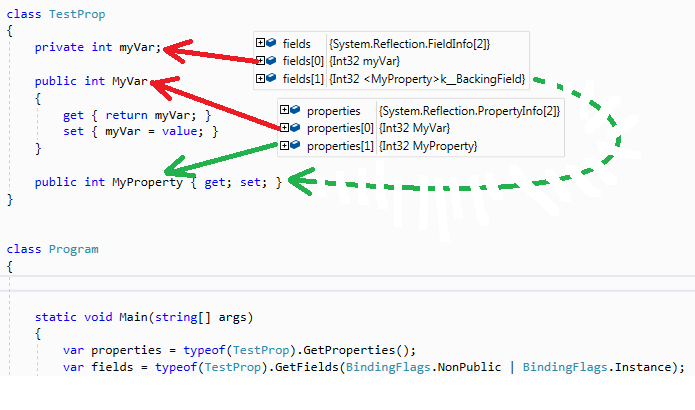
\includegraphics[width=\textwidth]{img/property_backing_field.png}
\end{frame}



\begin{frame}[fragile]
\frametitle{Javism -- gettery a settery}
\vfill
\begin{noblock}
\begin{lstlisting}[basicstyle=\small]
// String - klíčové slovo "string"
// atribut - místo vlastnosti
private String name;

// metoda jako getter a setter místo vlastosti
public String getName() {
    return name;
}

public void setName(String name) {
    this.name = name;
}
\end{lstlisting}
\end{noblock}
\vfill
\begin{yesblock}
\begin{lstlisting}[basicstyle=\small]
// "string"
// veřejná vlastnost - začíná velkým písmenem
public string Name { get; set; }
\end{lstlisting}
\end{yesblock}
\vfill
\end{frame}


\begin{frame}[fragile]
\begin{bitemize}{Vytváření vlastností ve Visual Studiu}
\item vlastnosti lze velmi efektivně vytvářet pomocí připravených code-snippets
\item []
\item \lstinline|prop<TAB><TAB>| -- vytvoří automaticky implementovanou vlastnost (TAB - přepíná mezi jednotlivými editovatelnými částmi)
\item \lstinline|propg<TAB><TAB>| -- stejné jako předchozí, ale je nastaveno \lstinline|private set|
\item \lstinline|propfull<TAB><TAB>| -- vytvoří vlastnost a backing atribut pro ní
\item \lstinline|propdp<TAB><TAB>| -- dependency property
\item \lstinline|propa<TAB><TAB>| -- attached dependency property
\end{bitemize}
\end{frame}


\kapitola{Metody}


\begin{frame}[fragile]
\frametitle{Metody}
\vfill
\begin{noteblock}{}
\begin{lstlisting}
[viditelnost] [modifikátory] typNávratovéHodnoty názevMetody([parametry]) těloMetody

těloMetody:
	=> výraz
	{ [příkazy] }
\end{lstlisting}
\end{noteblock}
\vfill
\begin{bitemize}{Modifikátory}
\item \lstinline|static| -- statická metoda
\item \lstinline|new| -- zakrývání metody z předka
\item \lstinline|virtual| -- virtuální metoda (polymorfizmus)
\item \lstinline|override| -- přetížená metoda (polymorfizmus)
\item \lstinline|abstract| -- abstraktní metoda (polymorfizmus)
\item \lstinline[morekeywords=async]|async| -- asynchronní metody
\end{bitemize}
\vfill
\end{frame}



\begin{frame}[fragile]
\frametitle{Metody -- příklad}
\vfill
\begin{yesblock}
\begin{lstlisting}[basicstyle=\small]
class Student
{
    public string Name { get; set; }

    public void SayHello()
    {
        Console.WriteLine($"Hello, I'm {Name}");
    }
}
\end{lstlisting}
\end{yesblock}
\vfill
\begin{yesblock}
\begin{lstlisting}[basicstyle=\small]
Student peter = new Student()
{
    Name = "Peter"
};

peter.SayHello();
\end{lstlisting}
\end{yesblock}
\vfill
\end{frame}




\begin{frame}[fragile]
\frametitle{Metody -- příklad zkráceného zápisu}
\vfill
\begin{yesblock}
\begin{lstlisting}[basicstyle=\small]
class Student
{
    public string Name { get; set; }

    public void SayHello() => Console.WriteLine($"Hello, I'm{Name}");
}
\end{lstlisting}
\end{yesblock}
\vfill
\end{frame}




\begin{frame}[fragile]
\frametitle{Metody -- výchozí hodnota parametru}
\begin{bitemize}{}
\item parametry mohou mít uvedenou výchozí hodnotu
\end{bitemize}
\vfill
\begin{yesblock}
\begin{lstlisting}[basicstyle=\small]
class MyMath
{
    public const double Pi = 3.141592;

    public static double GetPowerOfPi(int power = 1)
    {
        return Math.Pow(Pi, power);
    }
}
\end{lstlisting}
\end{yesblock}
\vfill
\begin{yesblock}
\begin{lstlisting}[basicstyle=\small]
double pi = MyMath.GetPowerOfPi();
double piSquare = MyMath.GetPowerOfPi(2);
\end{lstlisting}
\end{yesblock}
\end{frame}




\begin{frame}[fragile]
\frametitle{Metody -- ref}
\begin{bitemize}{}
\item parametr je možné předat odkazem (referencí)
\begin{itemize}
\item u parametru i u hodnoty argumentu je nutné uvést \lstinline|ref|
\end{itemize}

\end{bitemize}
\vfill
\begin{yesblock}
\begin{lstlisting}[basicstyle=\small]
class Toolkit
{
    public static void Increment(ref int value)
    {
        value++;
    }
}
\end{lstlisting}
\end{yesblock}
\vfill
\begin{yesblock}
\begin{lstlisting}[basicstyle=\small]
int intValue = 0;
Toolkit.Increment(ref intValue);
Console.WriteLine($"{intValue}");
\end{lstlisting}
\end{yesblock}
\end{frame}



\begin{frame}[fragile]
\frametitle{Metody -- out}
\begin{bitemize}{}
\item parametr může být výstupní
\begin{itemize}
\item u parametru i u hodnoty argumentu je nutné uvést \lstinline|out|
\end{itemize}

\end{bitemize}
\vfill
\begin{yesblock}
\begin{lstlisting}[basicstyle=\small]
class AuthenticationService
{
    public static bool Authentize(string password, out string username)
    {
        if (password == "secr3tP4ssw0rd!")
        {
            username = "admin";
            return true;
        }

        username = null;
        return false;
    }
}
\end{lstlisting}
\end{yesblock}
\end{frame}

\begin{frame}[fragile]
\frametitle{Metody -- out}
\vfill
\begin{yesblock}
\begin{lstlisting}[basicstyle=\small]
string username;
if(AuthenticationService.Authentize("password", out username))
{
    Console.WriteLine($"Authenticated as {username}");
}
\end{lstlisting}
\end{yesblock}
\vfill
\begin{yesblock}
\begin{lstlisting}[basicstyle=\small]
// C# 7 - podporuje deklarovat proměnnou v místě volání
if(AuthenticationService.Authentize("password", out string username))
{
    Console.WriteLine($"Authenticated as {username}");
}
\end{lstlisting}
\end{yesblock}
\vfill
\end{frame}




\nezkouskove

\begin{frame}[fragile]
\frametitle{Metody -- params}
\begin{bitemize}{}
\item je možné volat metodu s libovolným počtem parametrů (stejného typu)
\begin{itemize}
\item předáváno jako parametr typu pole s mod. \lstinline|params|
\item \lstinline|params| parametr musí být uveden jako poslední v seznamu parametrů
\end{itemize}

\end{bitemize}
\vfill
\begin{yesblock}
\begin{lstlisting}[basicstyle=\small]
public static int SumArguments(params int[] arguments)
{
    int sum = 0;
    foreach (var item in arguments)
    {
        sum += item;
    }

    return sum;
}
\end{lstlisting}
\end{yesblock}
\vfill
\begin{yesblock}
\begin{lstlisting}[basicstyle=\small]
int result = Summer.SumArguments(10, 20, 30, 40, 50, 60, 70);
\end{lstlisting}
\end{yesblock}
\end{frame}





\begin{frame}[fragile]
\frametitle{Metody -- pojmenované argumenty}
\begin{bitemize}{}
\item při volání metody je možné specifikovat argumenty v libovolném pořadí, pokud je uveden jejich název
\begin{itemize}
\item zapisuje se jako: \lstinline|názevParametru: hodnota|
\end{itemize}

\end{bitemize}
\vfill
\begin{yesblock}
\begin{lstlisting}[basicstyle=\small]
public static void AddProduct(string productName, int count = 1, 
    double weight = 0, string description = "")
\end{lstlisting}
\end{yesblock}
\vfill
\begin{yesblock}
\begin{lstlisting}[basicstyle=\small]
AddProduct("Toy", 10, 1.2, "Kid's toy");
AddProduct("Toy", count: 10, weight: 1.2);
AddProduct("Toy", description: "Kid's toy", count: 10);
// od C# 7.2:
AddProduct(productName: "Toy", 10, description: "Kid's toy"); 
\end{lstlisting}
\end{yesblock}
\end{frame}




\begin{frame}[fragile]
\frametitle{Metody -- ref return}

\begin{bitemize}{}
\item z metody je možné vracet referenci (C\# 7, mod. \lstinline|ref|)
\end{bitemize}
\vfill
\begin{yesblock}
\begin{lstlisting}[basicstyle=\small]
public static ref int FindGreaterThan(int[] array, int condition)
{
    for (int i = 0; i < array.Length; i++)
        if (array[i] > condition)
            return ref array[i];

    throw new Exception("Not found");
}
\end{lstlisting}
\end{yesblock}
\vfill
\begin{yesblock}
\begin{lstlisting}[basicstyle=\small]
int[] array = { 1, 2, 5, 15, 32, 64 };
Console.WriteLine($"{string.Join(" ", array)}");
ref int value = ref FindGreaterThan(array, 10);
value += 100;
Console.WriteLine($"{string.Join(" ", array)}");
\end{lstlisting}
\end{yesblock}
\end{frame}





\begin{frame}[fragile]
\frametitle{Metody -- rozšiřující (extension) metody}

\begin{bitemize}{}
\item (statická) metoda se tváří jako (instanční) metoda jiné třídy
\begin{itemize}
\item rozšířená třída je uvedena jako první parametr metody s mod. \lstinline|this|
\item metoda se volá přímo nad objektem rozšířené třídy
\end{itemize}

\item poprvé masivně použito pro realizaci LINQ
\end{bitemize}
\vfill
\begin{yesblock}
\begin{lstlisting}[basicstyle=\small]
class Student
{
  public string Name { get; set; }
}

static class StudentExtension
{
  public static void SayHello(this Student student, string weather)
  {
    Console.WriteLine($"Hello, I'm {student.Name} and it's {weather}");
  }
}
\end{lstlisting}
\end{yesblock}
\end{frame}

\begin{frame}[fragile]
\frametitle{Metody -- rozšiřující (extension) metody}
\begin{yesblock}
\begin{lstlisting}[basicstyle=\small]
Student student = new Student()
{
    Name = "Peter"
};

student.SayHello("sunny");
//Hello, I'm Peter and it's sunny
\end{lstlisting}
\end{yesblock}
\end{frame}


\zkouskove

\hkapitola{Objektové typy -- dědičnost, polymorfizmus}

\kapitola{Dědičnost}

\begin{frame}[fragile]
\begin{bitemize}{Dědičnost, polymorfizmus}
\item jednoduchá dědičnost -- je možné dědit z jednoho předka (Java)
\begin{itemize}
\item syntaxe připomíná C++
\item pokud není specifikován předek, třída automaticky dědí z~\lstinline|System.Object|
\end{itemize}
\item vícenásobná realizace rozhraní (Java)
\item explicitní rozlišování polymorfních metod -- časná/pozdní vazba (C++)
\end{bitemize}
\end{frame}



\begin{frame}[fragile]
\begin{bitemize}{Konstrukce objektu}
\item \lstinline|new System.Windows.Forms.Form()|
\item proces postupného volání konstruktorů
\begin{itemize}
\item \lstinline|System.Object|
\item \lstinline|System.MarshalByRefObject|
\item \lstinline|System.ComponentModel.Component|
\item \lstinline|System.Windows.Forms.Control|
\item \lstinline|System.Windows.Forms.ScrollableControl|
\item \lstinline|System.Windows.Forms.ContainerControl|
\item \lstinline|System.Windows.Forms.Form|
\end{itemize}
\item poté je objekt zkonstruován a lze jej používat
\end{bitemize}
\end{frame}



\begin{frame}[fragile]
\frametitle{Dědičnost}
\begin{noteblock}{}
\begin{lstlisting}[basicstyle=\small]
[viditelnost] [modifikátory] class NazevTridy [dědičnostARozhraní] { 
	[složkyTřídy]...
}

dědičnostARozhraní:
	: [názevPředkaNeboRozhraní], ...
\end{lstlisting}
\end{noteblock}
\vfill
\begin{yesblock}
\begin{lstlisting}[basicstyle=\small]
class Person
{
    public string Name { get; set; }
}

class Student : Person
{
    public string StudentID { get; set; }
}
\end{lstlisting}
\end{yesblock}
\end{frame}



\begin{frame}[fragile]
\frametitle{Dědičnost -- příklady}
\begin{yesblock}
\begin{lstlisting}[basicstyle=\small]
class Student : Person, IComparable, ICloneable { }
class Student : IComparable { }
class Student : ICloneable, IComparable { }
\end{lstlisting}
\end{yesblock}
\vfill
\begin{noblock}
\begin{lstlisting}[basicstyle=\small]
class Student : Person, Object { }
class Student : Person, LivingEntity { }
\end{lstlisting}
\end{noblock}
\end{frame}



\begin{frame}[fragile]
\vfill
\begin{bitemize}{}
\item automaticky se volá konstruktor předka
\begin{itemize}
\item kompilátor umí volat pouze bezparametrický konstruktor
\end{itemize}
\end{bitemize}
\vfill
\begin{yesblock}
\begin{lstlisting}[basicstyle=\small]
class Person
{
  public Person() => Console.WriteLine("Person()");
  public Person(string name) => Console.WriteLine("Person(string)");
}

class Student : Person
{
  public Student() => Console.WriteLine("Student()");
  public Student(string netid) => Console.WriteLine("Student(string)")
}
\end{lstlisting}
\end{yesblock}
\vfill
\end{frame}


\begin{frame}[fragile]
\begin{yesblock}
\begin{lstlisting}[basicstyle=\small]
Student student = new Student();
// Person()
// Student()

Student studentWithParam = new Student("netid");
// Person()
// Student(string netid)
\end{lstlisting}
\end{yesblock}
\end{frame}


\begin{frame}[fragile]
\begin{noblock}
\begin{lstlisting}[basicstyle=\small]
class Person
{
  //public Person() => Console.WriteLine("Person()");
  public Person(string name) => Console.WriteLine("Person(string)");
}

// nelze zkompilovat - kompilátor neumí vytvořit objekt
class Student : Person
{
  public Student() => Console.WriteLine("Student()");
  public Student(string netid) => Console.WriteLine("Student(string)")
}
\end{lstlisting}
\end{noblock}
\end{frame}



\begin{frame}[fragile]
\begin{bitemize}{}
\item konstruktor předka lze zavolat pomocí \lstinline|: base([parametry])|
\end{bitemize}
\vfill
\begin{yesblock}
\begin{lstlisting}[basicstyle=\small]
class Person
{
    //public Person() => Console.WriteLine("Person()");
    public Person(string name) => Console.WriteLine("Person(string name)");
}

class Student : Person
{
    public Student() : base("unknown") 
    {
        Console.WriteLine("Student()");
    }

    public Student(string name, string netid) : base(name) 
        => Console.WriteLine("Student(string, string)");
}
\end{lstlisting}
\end{yesblock}
\end{frame}




\begin{frame}[fragile]
\begin{bitemize}{}
\item lze zavolat i jiný konstruktor z aktuální třídy \lstinline|: this([parametry])|
\end{bitemize}
\vfill
\begin{yesblock}
\begin{lstlisting}[basicstyle=\small]
class Student : Person
{
    public Student() : this("unknown", "unidentified") 
    { 
    }

    public Student(string name, string netid) : base(name) 
        => Console.WriteLine("Student(string, string)");
}
\end{lstlisting}
\end{yesblock}
\end{frame}



\kapitola{Polymorfizmus}



\begin{frame}[fragile]
\frametitle{Polymorfizmus}

\begin{bitemize}{Základní vlastnosti}
\item potomek může zastoupit předka
\begin{itemize}
\item všude kde je očekáván předek je možné dosadit potomka
\end{itemize}

\item potomek může metody předka zakrýt nebo přepsat
\begin{itemize}
\item v javě je automaticky uplatňováno přepsání (tzv. pozdní vazba)
\item v C++ je časná/pozdní vazba rozlišena modifikátorem u metody
\item v C\# je uplatněn systém podobný C++
\end{itemize}

\end{bitemize}
\end{frame}



\begin{frame}[fragile]
\begin{noblock}
\begin{lstlisting}[basicstyle=\small]
class Person
{
  public void DoWork() => Console.WriteLine("Person goes to job!");
}

class Student : Person
{
  // warning CS0108 - úmyslné zakrývání má být označeno new
  public void DoWork() => Console.WriteLine("Student goes to school!");
}
\end{lstlisting}
\end{noblock}
\vfill
\begin{yesblock}
\begin{lstlisting}[basicstyle=\small]
Person person = new Person();
person.DoWork(); // -> person goes to job

Student student = new Student();
student.DoWork(); // -> student goes to school

person = student;
@@person.DoWork();@@ // -> person goes to job 
\end{lstlisting}
\end{yesblock}
\end{frame}



\begin{frame}[fragile]
\begin{bitemize}{Zakrývání}
\item zakrývání znamená vytvoření metody se stejným názvem jako v předkovi
\begin{itemize}
\item tato metoda, ale nemá polymorfní chování
\item metodu je nutné volat přímo nad instancí potomka, jinak se její kód nepoužije
\item kompilátor vyžaduje označování těchto metod klíčovým slovem \lstinline|new|
\end{itemize}
\end{bitemize}
\vfill
\begin{yesblock}
\begin{lstlisting}[basicstyle=\small]
class Person
{
  public void DoWork() => Console.WriteLine("Person goes to job!");
}

class Student : Person
{
  public new void DoWork() => Console.WriteLine("Student goes to school!");
}
\end{lstlisting}
\end{yesblock}
\end{frame}



\begin{frame}[fragile]
\begin{bitemize}{Polymorfizmus}
\item polymorfizmus umožňuje přetížit metodu v potomkovi
\begin{itemize}
\item taková metoda je použita, pokud pracujeme s typem potomka i předka
\item uplatňuje se tzv. pozdní vazba
\item v předkovi je nutné metodu označit \lstinline|virtual|
\end{itemize}
\end{bitemize}
\vfill
\begin{noblock}
\begin{lstlisting}[basicstyle=\small]
class Person
{
  public virtual void DoWork() => Console.WriteLine("Person");
}

class Student : Person
{
  // warning CS0114 - zakrývání virtual metody
  public void DoWork() => Console.WriteLine("Student");
}

// uvedený kód bude mít stejné chování jako předchozí dva slidy
// uplatněno je zakrývání / časná vazba!
\end{lstlisting}
\end{noblock}
\end{frame}



\begin{frame}[fragile]
\begin{bitemize}{Polymorfizmus}
\item polymorfizmus umožňuje přetížit metodu v potomkovi
\begin{itemize}
\item v předkovi je nutné metodu označit \lstinline|virtual|
\item v potomkovi je nutné metodu označit \lstinline|override|
\end{itemize}
\end{bitemize}
\vfill
\begin{yesblock}
\begin{lstlisting}[basicstyle=\small]
class Person
{
  public virtual void DoWork() => Console.WriteLine("Person");
}

class Student : Person
{
  public override void DoWork() => Console.WriteLine("Student");
}
\end{lstlisting}
\end{yesblock}
\vfill
\begin{yesblock}
\begin{lstlisting}[basicstyle=\small]
Person person = new Student();
person.DoWork(); // -> Student
\end{lstlisting}
\end{yesblock}
\end{frame}


\begin{frame}[fragile]
\begin{bitemize}{Rozpoznání typu objektu}
\item operátory \lstinline|is|, \lstinline|as|, \lstinline|(přetypování)|
\item metoda \lstinline|object.GetType()| a operátor \lstinline|typeof|
\item pattern matching (\lstinline|switch|)
\end{bitemize}
\vfill
\begin{bonusblock}{Polymorfizmus}
\begin{itemize}
\item C\# umožňuje hierarchii virtuálních metod přerušit a začít novou, je tak možné vytvořit metody
\begin{itemize}
\item prarodič -- \lstinline|virtual|
\item rodič -- \lstinline|override|
\item potomek -- \lstinline|new virtual|
\item \ldots
\end{itemize}

\end{itemize}
\end{bonusblock}
\end{frame}





\begin{frame}[fragile]
\begin{bitemize}{Abstraktní metody a třídy}
\item abstraktní metoda (\lstinline|abstract|) = virtuální metoda + nemá definici (tělo)
\begin{itemize}
\item musí být definována v abstraktní třídě
\end{itemize}
\item z abstraktní třídy nejde vytvořit objekt
\begin{itemize}
\item je nutné v potomkovi doplnit definici metody a vytvářet objekt potomka
\end{itemize}
\end{bitemize}
\vfill
\begin{yesblock}
\begin{lstlisting}[basicstyle=\small]
abstract class Person
{
    public abstract void DoWork();
}
\end{lstlisting}
\end{yesblock}
\vfill
\begin{noblock}
\begin{lstlisting}[basicstyle=\small]
Person person = new Person();
\end{lstlisting}
\end{noblock}
\end{frame}



\pkapitola{Rozhraní -- interface}



\begin{frame}[fragile]
\begin{bitemize}{Rozhraní}
\item značí předpis, který musí třída splnit
\begin{itemize}
\item třída může realizovat i více rozhraní
\item třída může rozhraní realizovat implicitně nebo explicitně
\end{itemize}
\item neobsahuje datové složky (atributy)
\item rozhraní nemůže definovat viditelnost složek
\item může obsahovat metody, vlastnosti, indexery, události
\end{bitemize}
\vfill
\begin{yesblock}
\begin{lstlisting}[basicstyle=\small]
interface IExample
{
    // Property
    int Property { get; set; }
    // Method
    void Method(int paramAlfa, int paramBeta);
    // Indexer
    int this[int param] { get; set; }
    // Event
    event ExampleEventHandler Event;
}
\end{lstlisting}
\end{yesblock}
\end{frame}




\begin{frame}[fragile]
\vfill
\begin{block}{}
Implicitní realizace rozhraní
\end{block}
\vfill
\begin{yesblock}
\begin{lstlisting}[basicstyle=\small]
interface IStringizable
{
    string Stringize();
}

class Student : IStringizable
{
    public string Name { get; set; }

    public string Stringize()
    {
        return Name;
    }
}
\end{lstlisting}
\end{yesblock}
\vfill
\end{frame}


\begin{frame}[fragile]
\vfill
\begin{bitemize}{Implicitní realizace rozhraní}
\item obdobné chování jako v Javě
\item metody rozhraní lze volat přímo nad objektem realizující třídy nebo po přetypování
\end{bitemize}
\vfill
\begin{yesblock}
\begin{lstlisting}[basicstyle=\small]
Student student = new Student();
var a = student.Stringize();

IStringizable istringizable = student;
var b = istringizable.Stringize();
\end{lstlisting}
\end{yesblock}
\vfill
\end{frame}







\begin{frame}[fragile]
\vfill
\begin{block}{}
Explicitní realizace rozhraní
\end{block}
\vfill
\begin{yesblock}
\begin{lstlisting}[basicstyle=\small]
interface IStringizable
{
    string Stringize();
}

class Student : IStringizable
{
    public string Name { get; set; }

    string IStringizable.Stringize() // <- uvedení názvu rozhraní před název metody
    {
        return Name;
    }
}
\end{lstlisting}
\end{yesblock}
\vfill
\end{frame}


\begin{frame}[fragile]
\begin{bitemize}{Explicitní realizace rozhraní}
\item nemá obdobu v Javě nebo C++
\item metody rozhraní lze volat pouze nad typem rozhraní
\item tento způsob realizace lze využít k rozlišení rozhraní, které mají složky se stejným identifikátorem
\end{bitemize}

\begin{yesblock}
\begin{lstlisting}[basicstyle=\small]
Student student = new Student();
// error CS1061
// var a = student.Stringize();

IStringizable istringizable = student;
var b = istringizable.Stringize();
\end{lstlisting}
\end{yesblock}
\end{frame}







\begin{frame}[fragile]
\begin{yesblock}
\begin{lstlisting}[basicstyle=\small]
interface IDrawable
{
    void Draw();
}

interface ISurface
{
    void Draw();
}

class Rectangle : IDrawable, ISurface
{
    public void Draw()
    {
        // ...
    }
}
\end{lstlisting}
\end{yesblock}
\vfill
\begin{bitemize}{}
\item implicitní realizace
\item obě rozhraní volají stejnou metodu \lstinline|Draw()|
\end{bitemize}
\end{frame}


\begin{frame}[fragile]
\begin{yesblock}
\begin{lstlisting}
interface IDrawable { void Draw(); }
interface ISurface { void Draw(); }

class Rectangle : IDrawable, ISurface
{
    public void Draw()
    {
        // ISurface
    }

    void IDrawable.Draw()
    {
        // IDrawable
    }
}
\end{lstlisting}
\end{yesblock}
\vfill
\begin{bitemize}{}
\item kombinace implicitní a explicitní realizace
\end{bitemize}
\end{frame}




\begin{frame}[fragile]
\begin{yesblock}
\begin{lstlisting}
interface IDrawable { void Draw(); }
interface ISurface { void Draw(); }

class Rectangle : IDrawable, ISurface
{
    void ISurface.Draw()
    {
        // ISurface
    }

    void IDrawable.Draw()
    {
        // IDrawable
    }
}
\end{lstlisting}
\end{yesblock}
\vfill
\begin{bitemize}{}
\item obě rozhraní používají explicitní realizaci
\end{bitemize}
\end{frame}


% 3
%
\hkapitola{Delegáty, události}

\begin{frame}[fragile]
\begin{bitemize}{Delegát}
\item \textbf{definuje datový typ} představující \textit{ukazatel na metodu}
\item typově bezpečný, bezpečné volání, \textbf{hodnotový typ}
\item instance delegátu (proměnná typu delegát) může obsahovat 0, 1 nebo více ukazatelů na metodu shodného předpisu
\end{bitemize}
\vfill
\begin{noteblock}{definice delegátu -- nového datového typu}
\begin{lstlisting}
delegate typNávratovéHodnoty názevTypuDelegátu([parametryMetody]);
\end{lstlisting}
\end{noteblock}
\vfill
\begin{yesblock}
\begin{lstlisting}
delegate void SimpleDelegate();
delegate int ReturnDelegate();
delegate int FunctionalDelegate(int a, int b);
\end{lstlisting}
\end{yesblock}
\vfill
\begin{bitemize}{}
\item název delegátu by se měl skládat z 
\begin{itemize}
\item vlastního popisu funkce
\item koncovky \lstinline|Callback| -- u obecného použití
\item koncovky \lstinline|EventHandler| -- u událostí
\end{itemize}

\end{bitemize}
\end{frame}





\begin{frame}[fragile]
\frametitle{Základní použití delegátu}
\begin{yesblock}
\begin{lstlisting}
delegate int CalculateCallback(); // definice delegáta

class Program
{
    static int CalculateStatic() => 1;  // statická metoda
    int CalculateInstance() => 2;       // instanční metoda

    static void Main(string[] args)
    {
        // vytvoření objektů delegátů
        CalculateCallback calculateStatic = CalculateStatic;
        CalculateCallback calculateInstance = (new Program()).CalculateInstance;

        var rs = calculateStatic();
        var ri = calculateInstance();
        Console.WriteLine($"{rs} {ri}");
    } }
\end{lstlisting}
\end{yesblock}
\end{frame}





\begin{frame}[fragile]
\frametitle{Vícenásobný delegát}
\begin{yesblock}
\begin{lstlisting}
delegate void OutputCallback();

class Program
{
    void Out1() => Console.WriteLine("1");
    void Out2() => Console.WriteLine("2");
    void Out3() => Console.WriteLine("3");
    void Out4() => Console.WriteLine("4");

    static void Main(string[] args)
    {
        // ...
    }
}
\end{lstlisting}
\end{yesblock}
\end{frame}




\begin{frame}[fragile]
\frametitle{Vícenásobný delegát\ldots}
\begin{yesblock}
\begin{lstlisting}
var program = new Program();
OutputCallback cc = null;

cc = program.Out1;
cc += program.Out2; cc += program.Out3; cc += program.Out4;
cc(); // 1 2 3 4

cc -= program.Out2;
cc(); // 1 3 4 

cc += program.Out4;
cc(); // 1 3 4 4

cc = program.Out2;
cc(); // 2

cc -= program.Out2;
cc(); // NullReferenceException
\end{lstlisting}
\end{yesblock}
\end{frame}




\begin{frame}[fragile]
\frametitle{Bezpečné vyvolání delegátu}
\begin{yesblock}
\begin{lstlisting}
var program = new Program();
OutputCallback cc = null;

if (cc != null)
{
    cc();
    // nebo
    cc.Invoke();
}

// nebo

cc?.Invoke();
\end{lstlisting}
\end{yesblock}
\end{frame}




\begin{frame}[fragile]
\frametitle{Delegát jako hodnotový typ}
\begin{yesblock}
\begin{lstlisting}
OutputCallback firstDelegate = program.Out1;

// hodnotový typ - zkopíruje ukazatele
OutputCallback secondDelegate = firstDelegate;
// změna neovlivní firstDelegate
secondDelegate += program.Out2;

firstDelegate(); // 1
secondDelegate(); // 1 2
\end{lstlisting}
\end{yesblock}
\end{frame}





\begin{frame}[fragile]
\begin{bitemize}{Základní typy delegátů v C\# knihovně}
\item \lstinline|void Action()|
\item \lstinline|void Action<p1>(p1)| -- generický delegát, je možné dosadit libovolný typ parametrů
\item \lstinline|void Action<p1, p2>(p1, p2)|
\item \lstinline|return Func<return>()|
\item \lstinline|return Func<p1, return>(p1)|
\item \lstinline|return Func<p1, p2, return>(p1, p2)|
\item \lstinline|bool Predicate<p>(p)|
\end{bitemize}

\vfill

\begin{yesblock}
\begin{lstlisting}
delegate void Example1Callback(Person person, int value);
// je "ekvivalentním" typem
Action<Person, int>

delegate string Example2Callback(Student student);
Func<Student, string>
\end{lstlisting}
\end{yesblock}
\end{frame}





\begin{frame}[fragile]
\begin{bitemize}{Delegát může obsahovat}
\item ukazatel na statickou metodu
\item ukazatel na instanční metodu
\item ukazatel na anonymní metodu
\end{bitemize}
\end{frame}



\pkapitola{Anonymní metody}


\begin{frame}[fragile]
\begin{bitemize}{}
\item anonymní metoda -- původní syntaxe
\begin{itemize}
\item klíčové slovo \lstinline|delegate|
\item seznam parametrů metody
\item tělo metody
\end{itemize}
\end{bitemize}
\vfill
\begin{yesblock}
\begin{lstlisting}
delegate int TransformCallback(int value);

static void Main(string[] args)
{
    TransformCallback tc = delegate (int value)
    {
        return value + 1;
    };

    int result = tc(1);
    Console.WriteLine($"{result}"); // 2
}
\end{lstlisting}
\end{yesblock}
\end{frame}




\begin{frame}[fragile]
\begin{bitemize}{}
\item anonymní metoda -- lambda funkce / výraz
\begin{itemize}
\item \lstinline|([parametry]) => { příkazy }|
\end{itemize}
\end{bitemize}
\vfill
\begin{yesblock}
\begin{lstlisting}
TransformCallback tc = (int i) => {
    return i + 1;
};

// blok může být nahrazen pouze výrazem
tc = (int i) => i + 1;

// datové typy parametrů mohou být odvozeny
tc = (i) => i + 1;

// pokud je pouze jeden parametr není nutné uvádět závorky
tc = i => i + 1;

int result = tc(1);
Console.WriteLine($"{result}"); // 2
\end{lstlisting}
\end{yesblock}
\end{frame}







\begin{frame}[fragile]
\begin{bitemize}{Praktická ukázka použití delegátů a anonymních metod}
\item parametrizace chování obecných algoritmů
\item technologie LINQ
\end{bitemize}
\vfill
\begin{yesblock}
\begin{lstlisting}
List<int> values = new List<int>
{
    10, 2, 24, 32, 5, 674, 23, 9875, 12, 43, 43, 23
};

var result = values
    // vyber pouze hodnoty větší než 10
    .Where(v => v > 10)
    // seřaď hodnoty od nejmenší po největší
    .OrderBy(v => v)
    // každou hodnotu umocni na druhou
    .Select(v => v * v)
    // vrať výsledek jako List
    .ToList();
// result = 144 529 529 576 1024 1849 1849 454276 97515625
\end{lstlisting}
\end{yesblock}
\end{frame}



\pkapitola{Události}

\begin{frame}[fragile]
\begin{bitemize}{Události -- teoreticky}
\item realizuje návrhový vzor observer
\item umožňuje objektům sledovat změny stavu konkrétního objektu
\begin{itemize}
\item příklad -- časovač nabídne událost Tik, která nastane vždy jednou za sekundu
\item konzole / grafické rozhraní se přihlásí (metodu PrintTime) k odběru Tiků
\item časovač odpočítá sekundu a vyvolá událost Tik, dojde k vyvolání metody PrintTime
\end{itemize}

\end{bitemize}
\end{frame}



\begin{frame}[fragile]
\begin{yesblock}
\begin{lstlisting}
static void Main(string[] args)
{
	// vytvoř časovač a spusť ho
    Timer t = new Timer();
    // nastav obslužnou metodu události
    t.Tick += TimerTickHandler;

    // ... program běží do stisku klávesy ...
    // Tick! Tick! Tick!

    Console.ReadKey();
}

private static void TimerTickHandler(object sender, EventArgs eventArgs)
{
    Console.WriteLine("Tick!");
}
\end{lstlisting}
\end{yesblock}
\end{frame}



\begin{frame}[fragile]
\begin{bitemize}{Událost -- event}
\item je složkou třídy
\item je \uv{proměnná} typu konkrétního delegáta
\item chová se velmi podobně jako normální proměnná typu delegát, ale
\begin{itemize}
\item vyvolat delegát může pouze definující třída
\item operátor = může použít pouze definující třída
\item ostatní třídy mohou používat +=, -= pro úpravu ukazatelů uložených v~delegátu
\end{itemize}
\end{bitemize}

\end{frame}






\begin{frame}[fragile]
\frametitle{Vytvoření vlastní události}
\vfill
\begin{bitemize}{1. delegát}
\item událost musí mít definovaný delegát, který definuje parametry události
\begin{itemize}
\item navratová hodnota \lstinline|void|
\item název delegátu končí \lstinline|EventHandler|
\item parametry metody
\begin{itemize}
\item \lstinline|object sender| -- kdo vyvolal událost
\item \lstinline|EventArgs eventArgs| -- parametry události (objekt \lstinline|EventArgs| nebo potomek této třídy)
\end{itemize}
\end{itemize}
\end{bitemize}
\vfill
\begin{yesblock}
\begin{lstlisting}
delegate void TickEventHandler(object sender, EventArgs eventArgs);
\end{lstlisting}
\end{yesblock}
\vfill
\end{frame}




\begin{frame}[fragile]
\vfill
\begin{bitemize}{2. událost}
\item ve třídě vytvoříme událost
\begin{itemize}
\item od běžné proměnné typu delegát se odlišuje klíčovým slovem \lstinline|event|
\end{itemize}
\end{bitemize}
\vfill
\begin{yesblock}
\begin{lstlisting}
class Timer
{
    public event TickEventHandler Tick;

    // ...
}
\end{lstlisting}
\end{yesblock}
\vfill
\end{frame}




\begin{frame}[fragile]
\begin{bitemize}{3. metoda pro vyvolání události}
\item ve třídě vytvoříme pomocnou metodu \lstinline|OnEvent...|
\begin{itemize}
\item bezpečně vyvolává událost
\item může být \lstinline|protected virtual| nebo i \lstinline|private| dle použití
\end{itemize}
\end{bitemize}
\vfill
\begin{yesblock}
\begin{lstlisting}
protected virtual void OnTick(EventArgs eventArgs)
{
    Tick?.Invoke(this, eventArgs);
}
\end{lstlisting}
\end{yesblock}
\vfill
\begin{oldblock}
\begin{lstlisting}
protected virtual void OnTick(EventArgs eventArgs)
{
    TickEventHandler handlers = Tick;
    if (handlers != null)
        handlers(this, eventArgs);
}
\end{lstlisting}
\end{oldblock}
\end{frame}







\begin{frame}[fragile]
\vfill
\begin{bitemize}{4. kód vyvolávající událost}
\item doplníme kód, který událost vyvolá
\end{bitemize}
\vfill
\begin{yesblock}
\begin{lstlisting}
public Timer()
{
    Thread t = new Thread(TimingThread);
    t.IsBackground = true;
    t.Start();
}

private void TimingThread()
{
    while (true)
    {
        Thread.Sleep(1000);

        OnTick(new EventArgs()); // <- vyvolej událost
    }
}
\end{lstlisting}
\end{yesblock}
\vfill
\end{frame}




\begin{frame}[fragile]
\vfill
\begin{bitemize}{5. použití události}
\item vně třídy nastavíme handler a událost zachytíme
\end{bitemize}
\vfill
\begin{yesblock}
\begin{lstlisting}
static void Main(string[] args)
{
	// vytvoř časovač a spusť ho
    Timer t = new Timer();
    // nastav obslužnou metodu události
    t.Tick += TimerTickHandler;

    // Tick! Tick! Tick!

    Console.ReadKey();
}

private static void TimerTickHandler(object sender, EventArgs eventArgs) =>
    Console.WriteLine("Tick!");
\end{lstlisting}
\end{yesblock}
\vfill
\end{frame}





\begin{frame}[fragile]
\vfill
\begin{bitemize}{Událost jako vlastnost}
\item událost může být definována jako vlastnost
\item vlastnost pak nabízí akce \lstinline|add| a \lstinline|remove| pro zpracování operátorů +=, -=
\end{bitemize}
\vfill
\begin{yesblock}
\begin{lstlisting}
private TickEventHandler tick;
public event TickEventHandler Tick
{
    add { tick += value; }
    remove { tick -= value; }
}
\end{lstlisting}
\end{yesblock}
\vfill
\end{frame}

%
\hkapitola{Výjimky}

\begin{frame}[fragile]

\begin{bitemize}{Výjimky}
\item slouží k ošetření chybových stavů v programu
\item systém je velmi podobný Javě
\item[]
\item vyvolání výjimky \lstinline|throw ...|
\item zachycení a zpracování výjimky \lstinline|try - catch - finally|
\item výjimky odvozeny od základní třídy \lstinline|System.Exception|
\item[]
\item nezachycená výjimka se šíří z metody dále
\begin{itemize}
\item na nejvyšší úrovni způsobí pád programu s chybovým hlášením
\end{itemize}

\end{bitemize}

\end{frame}




\begin{frame}[fragile]
\vfill
\begin{bitemize}{Vyvolání výjimky}
\item \lstinline|throw objektVýjimky|
\end{bitemize}
\vfill
\begin{yesblock}
\begin{lstlisting}
static void ComplexCalculation()
{
    throw new InvalidOperationException("broken toe");
}
\end{lstlisting}
\end{yesblock}
\vfill
\end{frame}



\begin{frame}[fragile]
\begin{bitemize}{Zachycení výjimky}
\item \lstinline|catch (typVýjimky názevProměnné)|
\end{bitemize}
\vfill
\begin{yesblock}
\begin{lstlisting}
try
{
    Console.WriteLine("pre throw");
    ComplexCalculation();
    Console.WriteLine("post throw");
}
catch (Exception ex)
{
    Console.Error.WriteLine(ex.Message);
}
\end{lstlisting}
\end{yesblock}
\end{frame}



\begin{frame}[fragile]
\begin{bitemize}{Zachycení výjimky -- univerzální catch}
\item \lstinline|catch|
\end{bitemize}
\vfill
\begin{yesblock}
\begin{lstlisting}
try
{
    Console.WriteLine("pre throw");
    ComplexCalculation();
    Console.WriteLine("post throw");
}
catch 
{
    Console.Error.WriteLine("catched something");
}
\end{lstlisting}
\end{yesblock}
\end{frame}


\begin{frame}[fragile]
\begin{bitemize}{Blok finally}
\item \lstinline|finally| -- nepovinné, blok je proveden vždy
\end{bitemize}
\vfill
\begin{yesblock}
\begin{lstlisting}
try
{
    Console.WriteLine("pre throw");
    ComplexCalculation();
    Console.WriteLine("post throw");
}
catch (Exception ex)
{
    Console.Error.WriteLine(ex.Message);
}
finally
{
    Console.WriteLine("finally");
}
\end{lstlisting}
\end{yesblock}
\end{frame}





\begin{frame}[fragile]
\frametitle{Třída System.Exception}
\begin{noteblock}{}
\begin{lstlisting}
public class Exception : ISerializable, _Exception
{
    public Exception();
    public Exception(string message);
    public Exception(string message, Exception innerException);

    public virtual string Source { get; set; }
    public virtual string HelpLink { get; set; }
    public virtual string StackTrace { get; }
    public MethodBase TargetSite { get; }
    public Exception InnerException { get; }
    public virtual string Message { get; }
    public int HResult { get; protected set; }
    public virtual IDictionary Data { get; }
    
    // ...
}
\end{lstlisting}
\end{noteblock}

\end{frame}



\begin{frame}[fragile]
\frametitle{Potomci třídy System.Exception}
\begin{noteblock}{}
\begin{itemize}
\item \lstinline|SystemException|
\item \lstinline|ApplicationException|
\item[]
\item \lstinline|IndexOutOfRangeException|
\item \lstinline|NullReferenceException|
\item \lstinline|AccessViolationException|
\item \lstinline|InvalidOperationException|
\item \lstinline|ArgumentException|
\item \lstinline|ArgumentNullException|
\item \lstinline|ArgumentOutOfRangeException|
\item \lstinline|ArithmeticException|
\item \lstinline|IndexOutOfRangeException|
\item \ldots
\end{itemize}
\end{noteblock}

\end{frame}




\begin{frame}[fragile]
\begin{bitemize}{Řízené použití prostředků pomocí try -- finally}
\item konstrukci \lstinline|try - finally| lze využít pro řízený přístup k prostředkům
\item blok \lstinline|finally| je proveden i v případě výskytu libovolné výjimky uvnitř \lstinline|try| bloku a je tak možné uklidit prostředky
\item rozhraní \lstinline|IDisposable| slouží k uvolnění těchto prostředků
\end{bitemize}
\vfill
\begin{yesblock}
\begin{lstlisting}
{
    Font font1 = new Font("Arial", 10.0f);
    try
    {
        byte charset = font1.GdiCharSet;
    }
    finally
    {
        if (font1 != null)
            ((IDisposable)font1).Dispose();
    }
}
\end{lstlisting}
\end{yesblock}
\end{frame}


\begin{frame}[fragile]
\vfill
\begin{bitemize}{Řízené použití prostředků pomocí try -- finally}
\item pro zjednodušení C\# nabízí ekvivalentní konstrukci \lstinline|using(...) { ... }|
\end{bitemize}
\vfill
\begin{yesblock} 
\begin{lstlisting}
using (Font font1 = new Font("Arial", 10.0f))
{
    byte charset = font1.GdiCharSet;
}
\end{lstlisting}
\end{yesblock}
\vfill
\begin{bitemize}{}
\item \lstinline|using| lze vnořovat nebo lze deklarovat více řízených proměnných najednou
\end{bitemize}
\vfill
\begin{yesblock}
\begin{lstlisting}
using (Font font3 = new Font("Arial", 10.0f),
            font4 = new Font("Arial", 10.0f))
{
    // Use font3 and font4.
}
\end{lstlisting}
\end{yesblock}
\end{frame}


\begin{frame}[fragile]
\begin{bitemize}{Kdy používat using}
\item nad objekty realizující rozhraní \lstinline|IDisposable|
\item \lstinline|System.IO, System.Net| -- třídy realizující operace se soubory/síťovými proudy
\item \lstinline|System.Data| -- třídy realizující databázové připojení a operace
\item \lstinline|System.Drawing| -- třídy popisující grafické objekty
\item \lstinline|System.Windows.Forms.Control| -- WinForms prvky
\item \ldots
\end{bitemize}
\end{frame}



%\hkapitola{Přetěžování operátorů}

\begin{frame}[fragile]
\vfill
\begin{bitemize}{Přetěžování operátorů}
\item podobně jako C++ lze v C\# přetěžovat operátory u svých objektových typů
\item množina přetížitelných operátorů je oproti C++ menší
\item syntax a pravidla pro přetěžování jsou striktnější a snaží se zamezit problémům
\begin{itemize}
\item např. není možné přetížit == bez přetížení !=
\end{itemize}

\end{bitemize}
\vfill
\begin{bitemize}{Přetížitelné operátory}
\item \lstinline|- ! ~ ++ -- true false|
\item \lstinline|- * / % & ^ | | \lstinline| << >> == != > < >= <=|
\item konverzní operátory
\item \lstinline|[ ]| (indexery)
\end{bitemize}
\vfill
\end{frame}


\nezkouskove

\begin{frame}[fragile]
\frametitle{Přetížení oprerátoru}
\vfill
\begin{noteblock}{}
\begin{lstlisting}
public static typ operator symbol ( parametry ) tělo
\end{lstlisting}
\end{noteblock}
\vfill
\begin{bitemize}{}
\item parametry
\begin{itemize}
\item unární operátor -- jeden parametr
\item binární operátor -- dva parametry
\end{itemize}

\item logické dvojice -- vždy je nutné přetížit oba operátory naráz
\begin{itemize}
\item \lstinline|== !=|
\item \lstinline|< >|
\item \lstinline|<= >=|
\item \lstinline|true false|
\end{itemize}

\item inkremetace/dekremetace se přetěžuje jednou metodou, kompilátor ji automaticky použije pro prefixovou i postfixovou variantu
\item operátory \lstinline|true,false| umožňují dát objekt přímo do výrazů očekávající logickou hodnotu (\lstinline|if, while, ...|)

\end{bitemize}
\vfill
\end{frame}




\begin{frame}[fragile]
\begin{yesblock}
\begin{lstlisting}
class Complex
{
    public double Re { get; set; }
    public double Im { get; set; }

    public static Complex operator +(Complex a, Complex b)
    {
        return new Complex()
        {
            Re = a.Re + b.Re,
            Im = a.Im + b.Im
        };
    }

    // ...
}
\end{lstlisting}
\end{yesblock}
\end{frame}




\begin{frame}[fragile]
\begin{yesblock}
\begin{lstlisting}
    public static bool operator ==(Complex a, Complex b)
    {
        return a.Re == b.Re && a.Im == b.Im;
    }

    public static bool operator !=(Complex a, Complex b)
    {
        return a.Re != b.Re || a.Im != b.Im;
    }
\end{lstlisting}
\end{yesblock}
\end{frame}




\begin{frame}[fragile]
\begin{yesblock}
\begin{lstlisting}
    public static Complex operator ++(Complex c)
    {
        return new Complex()
        {
            Re = c.Re + 1,
            Im = c.Im
        };
    }
\end{lstlisting}
\end{yesblock}
\end{frame}




\begin{frame}[fragile]
\frametitle{Přetížení oprerátoru -- konverzní operátory}
\vfill
\begin{noteblock}{}
\begin{lstlisting}
public static implicit operator cílovýTyp ( zdrojovýTyp parametr ) tělo
public static explicit operator cílovýTyp ( zdrojovýTyp parametr ) tělo
\end{lstlisting}
\end{noteblock}
\vfill
\begin{bitemize}{}
\item není možné zároveň definovat pravidla pro implicitní a explicitní konverzi
\item kompilátor tyto operátory volá při výrazech:
\begin{itemize}
\item implicitní
\begin{itemize}
\item \lstinline|cílovýTyp proměnná = objektZdrojovéhoTypu|
\end{itemize}

\item explicitní
\begin{itemize}
\item \lstinline|cílovýTyp proměnná  = (cílovýTyp)objektZdrojovéhoTypu|
\end{itemize}
\end{itemize}

\end{bitemize}
\vfill
\end{frame}




\begin{frame}[fragile]
\vfill
\begin{yesblock}
\begin{lstlisting}
    public static explicit operator double(Complex c)
    {
        return c.Re;
    }
\end{lstlisting}
\end{yesblock}
\vfill
\begin{yesblock}
\begin{lstlisting}
Complex c = new Complex()
{
    Re = 10,
    Im = 5
};

double realPart = (double)c;
Console.WriteLine($"{realPart}");
\end{lstlisting}
\end{yesblock}
\vfill
\end{frame}






\zkouskove

\begin{frame}[fragile]
\frametitle{Indexery}
\vfill
\begin{bitemize}{}
\item definují přetížení operátoru \lstinline|[ ]| pro přístup k prvkům/datům
\item definují se jako \textbf{instanční} (nestatické) \textbf{vlastnosti}
\end{bitemize}
\vfill
\begin{noteblock}{}
\begin{lstlisting}
[modifikátor] návratovýTyp this [ seznamParametrů ] deklaracePřístupovýchMetod
\end{lstlisting}
\end{noteblock}
\vfill
\begin{yesblock}
\begin{lstlisting}
class IndexerExample
{
    readonly int[] values = new int[] { 1, 2, 3, 4, 5, 6, 7, 8, 9, 10 };

    public int this[int index]
    {
        get => values[index];
    }
}
\end{lstlisting}
\end{yesblock}
\vfill
\end{frame}


\begin{frame}[fragile]
\frametitle{Indexery}
\vfill
\begin{bitemize}{}
\item je možné definovat několik různých přetížení indexerů s různými parametry
\item rozhraní mohou definovat indexery
\item indexer může data číst (\lstinline|get|) / zapisovat (\lstinline|set|) nebo provádět obojí
\end{bitemize}
\vfill
\begin{yesblock}
\begin{lstlisting}
var indexer = new IndexerExample();
int numberThree = indexer[2];
\end{lstlisting}
\end{yesblock}
\vfill
\end{frame}



\begin{frame}[fragile]
\begin{yesblock}
\begin{lstlisting}
class Table
{
    public Row this[int row]
    {
        get => GetRow(row);
        set => SetRow(row, value);
    }

    public string this[string identifier]
    {
        get => GetMetadata(identifier);
    }

    // ...

}
\end{lstlisting}
\end{yesblock}
\end{frame}

%\hkapitola{Preprocesor}


\begin{frame}[fragile]
\begin{bitemize}{Preprocesor}
\item podobně jako v C++ nabízí C\# preprocesor a několik příkazů, které se provedou před vlastní kompilací
\item možnosti jsou více omezené než v C++
\begin{itemize}
\item možnost podmíněné kompilace (dle definovaných symbolů preprocesoru)
\item možnost označovat část kódu (\lstinline|#region|) pro větší přehlednost v~editoru
\item možnost vyvolat chybu nebo varování při kompilaci části kódu 
\item možnost změnit číslo řádku nebo název souboru (\lstinline|#line|)
\item další možnosti dle kompilátoru (\lstinline|#pragma|)
\end{itemize}
\end{bitemize}

\end{frame}

\begin{frame}[fragile]
\vfill
\begin{bitemize}{\#define, \#undef}
\item definuje a ruší symboly (konstanty) preprocesoru
\item definice musí být na prvním místě v souboru
\item lze na nich založit podmíněnou kompilaci
\end{bitemize}
\vfill
\begin{yesblock}
\begin{lstlisting}
#define DEBUG
#undef TRACE
\end{lstlisting}
\end{yesblock}
\vfill
\end{frame}




\begin{frame}[fragile]
\vfill
\begin{bitemize}{\#if, \#elif, \#else, \#endif}
\item podmínkový blok v preprocesoru
\end{bitemize}
\vfill
\begin{yesblock}
\begin{lstlisting}[deletekeywords={if,else}]
#if (DEBUG && !MYTEST)
    Console.WriteLine("DEBUG is defined");
#elif (!DEBUG && MYTEST)
    Console.WriteLine("MYTEST is defined");
#elif (DEBUG && MYTEST)
    Console.WriteLine("DEBUG and MYTEST are defined");  
#else
    Console.WriteLine("DEBUG and MYTEST are not defined");
#endif
\end{lstlisting}
\end{yesblock}
\vfill
\end{frame}



\begin{frame}[fragile]
\vfill
\begin{bitemize}{ConditionalAttribute -- podmíněná kompilace pomocí atributu}
\item lze aplikovat na metody a třídy (pouze atributy)
\item pokud není podmínka splněna, daný objekt se nezkompiluje
\end{bitemize}
\vfill
\begin{yesblock}
\begin{lstlisting}
[Conditional("CONDITION1")]
public static void Method1(int x)
{
    Console.WriteLine("CONDITION1 is defined");
}

[Conditional("CONDITION1"), Conditional("CONDITION2")]  
public static void Method2()
{
    Console.WriteLine("CONDITION1 or CONDITION2 is defined");
}
\end{lstlisting}
\end{yesblock}
\vfill
\end{frame}



\begin{frame}[fragile]
\vfill
\begin{bitemize}{\#warning, \#error}
\item vyvolá varování nebo error v době kompilace na dané řádce
\end{bitemize}
\vfill
\begin{yesblock}
\begin{lstlisting}[deletekeywords={if,is}]
#define DEBUG  
class MainClass   
{  
    static void Main()   
    {  
#if DEBUG  
#warning DEBUG is defined  
#endif  
    }  
}  
\end{lstlisting}
\end{yesblock}
\vfill
\end{frame}


\begin{frame}[fragile]
\vfill
\begin{bitemize}{\#region, \#endregion}
\item označuje blok kódu, který spolu logicky souvisí
\item ve VS lze takový blok naráz zobrazit/skrýt pro větší přehlednost
\end{bitemize}
\vfill
\begin{yesblock}
\begin{lstlisting}
#region MyClass definition  
public class MyClass   
{  
    static void Main()   
    {  
    }  
}  
#endregion  
\end{lstlisting}
\end{yesblock}
\vfill
\end{frame}


%\hkapitola{Genericita}

\begin{frame}[fragile]
\begin{bitemize}{Genericita}
\item podobně jako v Javě je v C\# k dispozici genericita pro možnost \textbf{generického programování}
\item syntaxe velmi podobná Javě
\begin{itemize}
\item jinak se definují podmínky kovariance a kontravariance a omezující podmínky
\end{itemize}

\item Java genericitu realizuje technikou \uv{type erasure} (ve zkompilovaném kódu se genericita zahodí), C\# využívá \uv{reification} (\uv{zhmotnění typů} -- lze používat generické typy v reflexi i všude jinde)
\begin{itemize}
\item v důsledku existují třídy/rozhraní s genericitou a bez ní (\lstinline|IEnumerable| není to samé co \lstinline|IEnumerable<T>|)
\item metody lze přetěžovat s různými generickými parametry
\end{itemize}
\item \textbf{parametrem} generického typu může být \textbf{libovolný hodnotový i referenční typ} (tedy i primitivní datové typy)
\item vnořené typy automaticky dědí nařazené generické parametry
\end{bitemize}
\vfill


\end{frame}


\begin{frame}[fragile]
\begin{yesblock}
\begin{lstlisting}
class GenericHolder<T>
{
    public T Value { get; set; }
}
\end{lstlisting}
\end{yesblock}
\vfill
\begin{yesblock}
\begin{lstlisting}
GenericHolder<int> intHolder = new GenericHolder<int>();
intHolder.Value = 123;

Console.WriteLine(intHolder.Value);

// Chyba kompilace:
// intHolder.Value = "abcde";
\end{lstlisting}
\end{yesblock}
\end{frame}



\begin{frame}[fragile]
\vfill
\begin{bitemize}{Použití genericity}
\item generická třída/rozhraní -- za názvem třídy/rozhraní se uvede seznam typových parametrů
\begin{itemize}
\item \lstinline|class GenericClass<T> { }|
\end{itemize}

\item generická metoda -- obdobně za názvem metody
\begin{itemize}
\item \lstinline|public void GenericMethod<T>() { }|
\end{itemize}

\item generický delegát -- obdobně
\item pole a genericita -- jednorozměrná pole automaticky realizují rozhraní \lstinline|IList<T>|, použitelné pro čtení hodnot, modifikace vyvolají výjimku
\end{bitemize}
\vfill
\begin{bitemize}{Vytváření generických objektů/proměnných/\ldots}
\item při práci s generickými typy je nutné uvádět dosazené typy (\lstinline|Typ<KonkrétníTyp, JinýKonkrétníTyp>|)
\begin{itemize}
\item i při vytváření objektu, neexistuje tu obdoba Javovského diamond operátoru
\end{itemize}
\end{bitemize}
\vfill
\end{frame}


\begin{frame}[fragile]
\vfill
\begin{bitemize}{Pojmenování typových parametrů}
\item obecné \lstinline|T| v mnoha případech postačí
\item pokud je více typových parametrů, měly by být pojmenovány podle jejich účelu
\begin{itemize}
\item \lstinline|TÚčel, TJinýÚčel|
\item pokud je typový parametr omezen na určitý typ, mělo by jeho označení vycházet z omezujícího typu
\end{itemize}
\end{bitemize}
\vfill
\begin{yesblock}
\begin{lstlisting}
public interface ISessionChannel<TSession> { /*...*/ }
public delegate TOutput Converter<TInput, TOutput>(TInput from);
public class List<T> { /*...*/ }
\end{lstlisting}
\end{yesblock}
\vfill
\end{frame}



\begin{frame}[fragile]
\vfill
\begin{bitemize}{Omezení typových parametrů}
\item C\# umožňuje definovat omezení, které musí platit pro typový parametr
\item[] \lstinline[morekeywords={where}]|where T : omezeníTypovéhoParametru|
\end{bitemize}
\vfill
\begin{bitemize}{}
\item \lstinline|struct| -- musí být hodnotového typu (nezahrnuje nullable typy)
\item \lstinline|class| -- musí být referenčního typu (třída, rozhraní, delegát, pole)
\item \lstinline|new()| -- musí mít definovaný veřejný bezparametrický konstruktor
\item \lstinline|názevTřídy| -- musí být potomkem dané třídy
\item \lstinline|názevRozhraní| -- musí realizovat dané rozhraní
\item \lstinline|U| -- musí být stejného typu nebo potomkem jako obecný typ \lstinline|U|
\end{bitemize}
\vfill
\end{frame}


\begin{frame}[fragile]
\begin{yesblock}
\begin{lstlisting}[morekeywords={where}]
class OrderedList<T> where T : IComparable<T>
{
    // ...

    public void Add(T item)
    {
        if (item.CompareTo(...) > 0)
            // ...
    }
}
\end{lstlisting}
\end{yesblock}
\end{frame}


\begin{frame}[fragile]
\begin{bitemize}{}
\item je možné definovat více omezení na jeden typový parametr
\item je možné definovat omezení pro více typových parametrů
\end{bitemize}
\vfill
\begin{yesblock}
\begin{lstlisting}[morekeywords={where}]
class EmployeeList<T> where T : Employee, IEmployee, System.IComparable<T>, new()
{
    // ...
}
\end{lstlisting}
\end{yesblock}
\vfill
\begin{yesblock}
\begin{lstlisting}[morekeywords={where}]
class Base { }
class Test<T, U>
    where U : struct
    where T : Base, new() { }
\end{lstlisting}
\end{yesblock}
\end{frame}



\begin{frame}[fragile]
\begin{bitemize}{Inicializace proměnné typového parametru}
\item v obecném případě se může jednat o hodnotový i referenční typ
\begin{itemize}
\item hodnota \lstinline|null| je platná jen pro refereční typy
\item získat výchozí hodnotu pro daný typ je možné pomocí \lstinline|default(Typ)|
\end{itemize}
\end{bitemize}
\vfill
\begin{yesblock}
\begin{lstlisting}
class PtrCounter<T>
{
    public T Ptr { get; set; }
    public int References { get; set; }

    public PtrCounter()
    {
        Ptr = default(T);
        References = 0;
    }

    // ...
}
\end{lstlisting}
\end{yesblock}
\end{frame}

%\hkapitola{Jmenné prostory}

\begin{frame}[fragile]
\frametitle{Jmenné prostory}
\vfill
\begin{bitemize}{namespace}
\item stejně jako balíčky slouží k logickému oddělení kódu -- rozdělení na spolu související komponenty a \textbf{zamezení konfliktů jmen}
\item jmenné prostory na rozdíl od Java balíčků \textbf{nevyžadují přesnou organizaci na disku}
\item jmenné prostory je možné \textbf{libovolně vnořovat}
\end{bitemize}
\vfill
\begin{bitemize}{}
\item uvnitř jmenného prostoru jsou vidět složky definované v tomto jmenném prostoru
\item složky definované v jiném jmenném prostoru je nutné zpřístupnit užitím plné cesty a názvu komponenty nebo zpřístupnit jmenný prostor pomocí \lstinline|using|
\end{bitemize}
\vfill
\end{frame}



\begin{frame}[fragile]
\vfill
\begin{bitemize}{Definování jmenných prostorů}
\item jmenný prostor je možné definovat na globální úrovni nebo v jiném jmenném prostoru
\item [] \lstinline|namespace NázevJmennéhoProstoru { ... }|
\end{bitemize}
\vfill
\begin{yesblock}
\begin{lstlisting}
namespace Game
{
    // Game ...

    namespace Graphics
    {
        // Game.Graphics ...
    }
}
\end{lstlisting}
\end{yesblock}
\vfill
\end{frame}





\begin{frame}[fragile]
\vfill
\begin{bitemize}{Vnořené jmenné prostory}
\item u vnořených jmenných prostorů není nutné vytvářet N vnořených bloků \lstinline|namespace|, ale postačí uvést plnou cestu k jmennému prostoru 
\end{bitemize}
\vfill
\begin{yesblock}
\begin{lstlisting}
namespace Game.Graphics
{
    // Game.Graphics ...
}
\end{lstlisting}
\end{yesblock}
\end{frame}




\begin{frame}[fragile]
\frametitle{Použití jmenných prostorů -- definice}

\begin{yesblock}
\begin{lstlisting}
namespace First
{
    class FirstClass
    {
        public const int FirstConst = 1;
    }
}
\end{lstlisting}
\end{yesblock}
\end{frame}




\begin{frame}[fragile]
\frametitle{Použití jmenných prostorů -- zpřístupnění jiného jmenného prostoru}
\vfill
\begin{bitemize}{}
\item standardně je nutné uvést plnou \uv{cestu} k dané složce
\end{bitemize}
\vfill
\begin{yesblock}
\begin{lstlisting}
namespace Second
{
    class SecondClass
    {
        static void Method()
        {
            // FirstConst // error CS0103
            // FirstClass.FirstConst // error CS0103
            var v = First.FirstClass.FirstConst;
        }
    }
}
\end{lstlisting}
\end{yesblock}
\vfill
\end{frame}




\begin{frame}[fragile]
\frametitle{Použití jmenných prostorů -- using}
\vfill
\begin{bitemize}{}
\item pomocí \lstinline|using| lze zpřístupnit obsah jmenného prostoru do aktuálního kontextu
\end{bitemize}
\vfill
\begin{yesblock}
\begin{lstlisting}
using First;

namespace Second
{
    class SecondClass
    {
        static void Method()
        {
            var v = FirstClass.FirstConst;
        }
    }
}
\end{lstlisting}
\end{yesblock}
\vfill
\end{frame}






\begin{frame}[fragile]
\frametitle{Zpřístupnění statických položek -- using static}
\vfill
\begin{bitemize}{}
\item od C\# 6 existuje klauzule \lstinline|using static|, která umožňuje přímo pracovat se statickými složkami vybraného typu
\end{bitemize}
\vfill
\begin{yesblock}
\begin{lstlisting}
using static System.Math;

class ExampleUsingStaticClass
{
    static double CalculateCircleArea(double radius)
    {
        // bez using static:
        // return Math.PI * Math.Pow(radius, 2);
        
        return PI * Pow(radius, 2);
    }
}
\end{lstlisting}
\end{yesblock}
\vfill
\end{frame}

%%System.Collections
%ArrayList
%BitArray
%Hashtbake
%Queue
%SortedList
%Stack

%System.Collections.Generic
%Dictionary
%List

%SystemCollectionsConcurrent
%ConcurrentDictionary/Queue/Stack
%%BinaryReader - stream
%writer - stream
%bufferedstream - stream
%
%filestream
%memorystream
%
%streamreader - stream
%streamwriter - stream
%
%stringreader/writer - string
%
%Stream - abstract
%textreader/writer - abtstract class
%
%File,FileInfo
%Directory,DirectoryInfo
%Path

\hkapitola{Input/output}


\kapitola{Souborový systém}


\begin{frame}[fragile]
\begin{bitemize}{Abstrakce souborového systému}
\item Jmenný prostor \lstinline|System.IO|
\item Základní třídy:
\begin{itemize}
\item \lstinline|File| -- statická třída pro práci se soubory
\item \lstinline|Path| -- statická třída pro práci s cestami
\item \lstinline|Directory| -- statická třída pro práci s adresáři
\item[]
\item \lstinline|FileInfo| -- objekt představuje konkrétní soubor
\item \lstinline|DirectoryInfo| -- objekt představuje konkrétní adresář
\item \lstinline|DriveInfo| -- objekt představuje konkrétní jednotku

\end{itemize}

\end{bitemize}
\end{frame}




\begin{frame}[fragile]
\begin{yesblock}
\begin{lstlisting}
if (File.Exists(@".\file.txt"))
{
    // ...
}

FileInfo file = new FileInfo(@".\file.txt");
if (file.Exists)
{
    // ...
}
\end{lstlisting}
\end{yesblock}
\vfill
\begin{yesblock}
\begin{lstlisting}
FileStream fs = File.Create(@".\created.txt");
fs.Close();

FileStream fsInstance = new FileInfo(@".\created.txt").Create();
fsInstance.Close();
\end{lstlisting}
\end{yesblock}
\end{frame}




\begin{frame}[fragile]
\begin{yesblock}
\begin{lstlisting}
DirectoryInfo di = new DirectoryInfo(".\\");
foreach (FileInfo file in di.EnumerateFiles())
{
    Console.WriteLine($"{file.Name} - {file.Extension} - {file.LastAccessTime}");
}

/*
ConsoleApp1.exe - .exe - 05.02.2018 22:07:58
ConsoleApp1.exe.config - .config - 05.02.2018 22:07:58
ConsoleApp1.pdb - .pdb - 05.02.2018 22:07:58
created.txt - .txt - 11.03.2018 10:23:01
 */
\end{lstlisting}
\end{yesblock}
\vfill
\begin{yesblock}
\begin{lstlisting}
DirectoryInfo di = new DirectoryInfo(@".\nonExistentDirectory");
di.Create();

Console.WriteLine(di.FullName);
// C:\Users\<...>\ConsoleApp1\bin\Debug\nonExistentDirectory
\end{lstlisting}
\end{yesblock}
\end{frame}



\begin{frame}[fragile]
\begin{yesblock}
\begin{lstlisting}
DriveInfo di = new DriveInfo("C");

var sizeInGB = di.TotalSize / 1024 / 1024 / 1024;
var freeInGB = di.TotalFreeSpace / 1024 / 1024 / 1024;
var fs = di.DriveFormat;

Console.WriteLine($"{fs} - free {freeInGB} / {sizeInGB} GB");
// NTFS - free 125 / 432 GB
\end{lstlisting}
\end{yesblock}
\vfill
\begin{yesblock}
\begin{lstlisting}
DriveInfo[] drives = DriveInfo.GetDrives();
foreach (DriveInfo drive in drives)
{
    Console.WriteLine($"{drive.Name} - {drive.DriveFormat} - {drive.DriveType}");
}

// C:\ - NTFS - Fixed
// D:\ - NTFS - Fixed
\end{lstlisting}
\end{yesblock}
\end{frame}



\kapitola{Proudy}




\begin{frame}[fragile]
\vfill
\begin{bitemize}{Základní proudy pro práci se soubory, pamětí, \ldots}
\item knihovna využívá stejných principů jako Java
\item základní abstraktní třída \lstinline|Stream| reprezentuje datový proud
\begin{itemize}
\item potomci představují konkrétní použití -- \lstinline|FileStream|, \lstinline|MemoryStream|, \lstinline|NetworkStream|, \ldots
\item existuje zde řada dekorátorů -- \lstinline|BufferedStream|, \lstinline|DeflateStream|, \lstinline|GZipStream|, \lstinline|CryptoStream|, \ldots
\end{itemize}
\item pro realizaci textových přenosů slouží třídy \lstinline|StreamReader|, \lstinline|StreamWriter|
\begin{itemize}
\item binární přenosy \lstinline|BinaryReader|, \lstinline|BinaryWriter|
\end{itemize}
\end{bitemize}
\vfill
\begin{bitemize}{}
\item proudy je třeba korektně uzavírat, jinak může dojít ke ztrátě dat a prostředky mohou být dlouho blokovány
\item proudy typicky realizují \lstinline|IDisposable| rozhraní (lze využít konstrukci \lstinline|using|)
\end{bitemize}
\vfill
\end{frame}



\begin{frame}[fragile]
\vfill
\begin{bitemize}{Abstraktní třída Stream}
\item \lstinline|Position| -- vlastnost, pozice kurzoru
\item \lstinline|CanRead, CanWrite, CanSeek| -- vlastnosti
\item \lstinline|Seek| -- přesune kurzor v souboru
\item \lstinline|Read| -- čte pole bajtů
\item \lstinline|Write| -- zapisuje pole bajtů
\item \lstinline|ReadByte| -- čte bajt
\item \lstinline|WriteByte| -- zapisuje bajt
\item \lstinline|Close| -- uzavře proud
\end{bitemize}
\vfill
\begin{bitemize}{Potomci třídy Stream}
\item \lstinline|BaseStream| -- vlastnost, není definováno rozhraním, nemusí být u~všech
\end{bitemize}
\vfill
\end{frame}


\pkapitola{Zápis a čtení textových dat}


\begin{frame}[fragile]
\vfill
\begin{bitemize}{Zápis a čtení textových dat}
\item Třídy \lstinline|StreamWriter|, \lstinline|StreamReader|
\item pracují nad obecným proudem (soubor, paměť, síť, \ldots)
\item kódování znaků je volitelné
\begin{itemize}
\item výchozí kódování je UTF-8
\end{itemize}
\end{bitemize}
\vfill
\begin{bitemize}{Základní metody}
\item \lstinline|Write()| -- zápis znaku/znaků/hodnoty základních dat. typů
\item \lstinline|WriteLine()| -- zápis řádku textu
\item \lstinline|Read()| -- načtení znaku nebo pole znaků
\item \lstinline|ReadLine()| -- načtení řádku
\end{bitemize}
\vfill
\end{frame}




\begin{frame}[fragile]
\vfill
\begin{bitemize}{StreamWriter -- konstrukce}
\item \lstinline|StreamWriter(Stream stream)|
\item \lstinline|StreamWriter(string path)|
\item \lstinline|StreamWriter(Stream stream, Encoding encoding)|
\item \lstinline|StreamWriter(string path, bool append)|
\item \ldots
\end{bitemize}
\vfill
\begin{bitemize}{StreamReader -- konstrukce}
\item \lstinline|StreamReader(Stream stream)|
\item \lstinline|StreamReader(Stream stream, bool detectEncodingFromByteOrderMarks)|
\item \lstinline|StreamReader(Stream stream, Encoding encoding)|
\item \lstinline|StreamReader(Stream stream, Encoding encoding, bool detectEncodingFromByteOrderMarks)|
\item dtto se \lstinline|string path| \ldots
\end{bitemize}
\vfill
\end{frame}



\begin{frame}[fragile]
\frametitle{Zápis a čtení z textového souboru}
\begin{yesblock}
\begin{lstlisting}
using (StreamWriter writer = new StreamWriter(new FileStream("output.txt", FileMode.OpenOrCreate), Encoding.UTF8))
{
    writer.WriteLine("Hello World");
    writer.WriteLine("Příliš žluťoučký kůň úpěl ďábelské ódy");
}

using (var reader = new StreamReader("output.txt"))
{
    Console.WriteLine(reader.ReadLine());
    Console.WriteLine(reader.ReadLine());
}
\end{lstlisting}
\end{yesblock}
\end{frame}


\begin{frame}[fragile]
\frametitle{Základní metody StreamReader, StreamWriter}
\vfill
\begin{yesblock}
\begin{lstlisting}
writer.Write(123);
writer.Write(123.456);
writer.Write(true);
writer.Write(obj);
writer.WriteLine(dtto);
\end{lstlisting}
\end{yesblock}
\vfill
\begin{yesblock}
\begin{lstlisting}
int char = reader.Read();

char[] buffer = new char[100];
reader.Read(buffer, 0, buffer.Length);

string line = reader.ReadLine();

string tillTheEnd = reader.ReadToEnd();
\end{lstlisting}
\end{yesblock}
\vfill
\end{frame}






\begin{frame}[fragile]
\begin{bitemize}{Kódování textu}
\item Třída \lstinline|System.Text.Encoding|
\item Vlastnosti:
\begin{itemize}
\item \lstinline|ASCII| - ASCII kódování, bez podpory rozšířených znaků
\item \lstinline|BigEndianUnicode| -- UTF-16 Big Endian
\item \lstinline|Default| -- výchozí pro aktuální platformu (Windows - cp1250/windows-1250/iso-8859-2)
\item \lstinline|Unicode| -- UTF-16 Little Endian
\item \lstinline|UTF32| -- UTF-32 Little Endian
\item \lstinline|UTF7| -- UTF-7
\item \lstinline|UTF8| -- UTF-8
\end{itemize}
\item Statické metody
\begin{itemize}
\item \lstinline|Convert(...)| -- převede pole bajtů ze zadaného kódování do cílového
\item \lstinline|GetEncoding(...)| -- vrátí kódování podle označení nebo čísla kódové stránky
\item \lstinline|GetEncodings()| -- vrátí pole všech použitelných kódování
\end{itemize}

\end{bitemize}
\end{frame}



\begin{frame}[fragile]
\frametitle{Kódování textu}
\begin{yesblock}
\begin{lstlisting}
// zápis v UTF-16 Little Endian
using (StreamWriter sw = new StreamWriter(File.OpenWrite("unicode.txt"), Encoding.Unicode)) {
    sw.WriteLine("Příliš žluťoučký kůň úpěl dábělské ódy");
}

// false - nedetekuj kódování z BOM hlavičky souboru
// provede čtení v UTF-8
using (StreamReader sr = new StreamReader(File.OpenRead("unicode.txt"), false))
{
    Console.WriteLine(sr.ReadLine());
    // ??P Y?? l i a?  ~?l u e?o u
}
\end{lstlisting}
\end{yesblock}
\end{frame}



\pkapitola{Zápis a čtení binárních dat}



\begin{frame}[fragile]
\begin{bitemize}{Binární soubory}
\item pro práci s binárními soubory slouží třídy \lstinline|BinaryWriter|, \lstinline|BinaryReader|
\item nabízejí metody pro čtení a zápis všech primitivních datových typů
\item[]
\item C\# dále nabízí možnosti serializace nebo i možnost práce s unmanaged memory

\end{bitemize}
\end{frame}





\begin{frame}[fragile]
\frametitle{Zápis a čtení z binárních souborů}
\begin{yesblock}
\begin{lstlisting}
using (var writer = new BinaryWriter(new FileStream("binary.dat", FileMode.Create)))
{
    // write je přetížena pro všechny základní typy
    writer.Write(true);
    writer.Write(0x11223344);
    writer.Write(123.456);
    writer.Write('z');
    writer.Write("string");

    // a podporován je i blokový přenos pomocí pole bajtů
    byte[] buffer = new byte[16];
    writer.Write(buffer, 0, buffer.Length);
}
\end{lstlisting}
\end{yesblock}
\end{frame}


\begin{frame}[fragile]
\frametitle{Zápis a čtení z binárních souborů}
\begin{yesblock}
\begin{lstlisting}
using (var reader = new BinaryReader(new FileStream("binary.dat", FileMode.Open)))
{
    bool boolVar = reader.ReadBoolean();
    int intVar = reader.ReadInt32();
    double doubleVar = reader.ReadDouble();
    char charVar = reader.ReadChar();
    string strVar = reader.ReadString();

    byte[] buffer = new byte[16];
    reader.Read(buffer, 0, buffer.Length);
}
\end{lstlisting}
\end{yesblock}
\end{frame}



\nezkouskove

\begin{frame}[fragile]
\vfill
\begin{bonusblock}{~}
\begin{itemize}
\item ukázka použití unmanaged memory a marshallingu
\end{itemize}
\end{bonusblock}
\vfill
\begin{yesblock}
\begin{lstlisting}
// třída nemá ve výchozím chování pevnou strukturu, proto je třeba ji označit atributem
[StructLayout(LayoutKind.Sequential, CharSet = CharSet.Unicode)]
class Student
{
    // rovněž je možné specifikovat konkrétní způsob marshallingu jednotlivých datových složek
    [MarshalAs(UnmanagedType.ByValTStr, SizeConst = 50)]
    private string name;
    [MarshalAs(UnmanagedType.ByValTStr, SizeConst = 50)]
    private string lastName;
    [MarshalAs(UnmanagedType.I4)]
    private int id;

    // ...
}
\end{lstlisting}
\end{yesblock}
\vfill
\end{frame}


\begin{frame}[fragile]
\begin{yesblock}
\begin{lstlisting}
using (FileStream fs = File.OpenWrite("binary.dat"))
{
    Student student = new Student()
    {
        Name = "Petr",
        LastName = "Rychly",
        Id = 1234
    };

    var size = Marshal.SizeOf(student); // velikost struktury

    var ptr = Marshal.AllocHGlobal(size); // alokace unmanaged pole
    Marshal.StructureToPtr(student, ptr, false); 

    var bytes = new byte[size]; // managed pole pro uložení struktury
    Marshal.Copy(ptr, bytes, 0, size); // copy unmanaged -> managed
    Marshal.FreeHGlobal(ptr); // uvolnění pole

    fs.Write(bytes, 0, size);
}
\end{lstlisting}
\end{yesblock}
\end{frame}


\begin{frame}[fragile]
\begin{yesblock}
\begin{lstlisting}
using (FileStream fs = File.OpenRead("binary.dat"))
{
    Student student = new Student();

    var size = Marshal.SizeOf<Student>();

    var bytes = new byte[size];
    fs.Read(bytes, 0, size);

    var ptr = Marshal.AllocHGlobal(size);
    Marshal.Copy(bytes, 0, ptr, size);
    Marshal.PtrToStructure(ptr, student);
    Marshal.FreeHGlobal(ptr);

    Console.WriteLine($"{student.Name} {student.LastName} {student.Id}");
}
\end{lstlisting}
\end{yesblock}
\end{frame}


\zkouskove


\pkapitola{Paměťové proudy}


\begin{frame}[fragile]
\begin{bitemize}{Paměťové proudy}
\item realizovány třídou \lstinline|MemoryStream|
\item na pozadí používají pole bajtů (\lstinline|byte[]|), může být fixní délky nebo rozšířitelné
\item podporuje základní \lstinline|Write()| a \lstinline|Read()| operace
\item po ukončení zápisu lze pole získat pomocí met. \lstinline|ToArray()| nebo zapsat obsah do jiného proudu pomocí \lstinline|WriteTo(stream)|
\end{bitemize}
\vfill
\begin{yesblock}
\begin{lstlisting}
using (MemoryStream ms = new MemoryStream())
{
    for (int i = 0; i < 256; i++)
        ms.WriteByte((byte)i);

    using (FileStream fs = File.OpenWrite("bytes.dat"))
    {
        ms.WriteTo(fs);
    }
}
\end{lstlisting}
\end{yesblock}
\end{frame}



\kapitola{Příklad komprese a dekomprese}


\begin{frame}[fragile]
\begin{yesblock}
\begin{lstlisting}
string str = "Testování deflate komprese";
int randomLen = 1024 * 1024;

long originalLength = Encoding.Default.GetBytes(str).Length + randomLen;
Console.WriteLine($"Original len: {originalLength}");

using (var fileStream = File.OpenWrite("compressed.dat"))
{
    using (var deflateStream = new DeflateStream(fileStream, CompressionMode.Compress))
    {
        using (var stream = new StreamWriter(deflateStream))
        {
            stream.WriteLine(str);

            Random random = new Random();
            for (int i = 0; i < randomLen; i++)
                stream.Write((char)random.Next('a', 'z'));
}   }   }
\end{lstlisting}
\end{yesblock}
\end{frame}


\begin{frame}[fragile]
\begin{yesblock}
\begin{lstlisting}
long length = new FileInfo("compressed.dat").Length;
Console.WriteLine($"Compressed len: {length}");
Console.WriteLine($"Compression ratio: {length/(double)originalLength*100} %");

using (var fileStream = File.OpenRead("compressed.dat"))
{
    using (var deflateStream = new DeflateStream(fileStream, CompressionMode.Decompress))
    {
        using (var stream = new StreamReader(deflateStream))
        {
            Console.WriteLine(stream.ReadLine());
            Console.ReadKey();
            Console.WriteLine(stream.ReadLine());
} } }
// Original len: 1048602
// Compressed len: 664080
// Compression ratio: 63,3300337020147 %
\end{lstlisting}
\end{yesblock}
\end{frame}






\kapitola{Serializace}



\begin{frame}[fragile]
\begin{bitemize}{Serializace}
\item metoda pro převedení objektu(ů) do přenositelné podoby (textová/binární)
\item při serializaci je převáděn kompletní objektový graf
\item C\# podporuje několik základních druhů serializátorů
\begin{itemize}
\item binární formát 
\begin{itemize}
\item \lstinline|System.Runtime.Serialization.Formatters.Binary.BinaryFormatter|
\end{itemize}

\item XML
\begin{itemize}
\item \lstinline|System.Xml.Serialization.XmlSerializer|
\item \lstinline|System.Runtime.Serialization.DataContractSerializer|
\end{itemize}

\item SOAP
\begin{itemize}
\item \lstinline|System.Runtime.Serialization.Formatters.Soap.SoapFormatter|
\end{itemize}

\end{itemize}
\end{bitemize}
\end{frame}


\pkapitola{Binární / SOAP serializace}


\begin{frame}[fragile]
\begin{bitemize}{Birnání / SOAP serializace}
\item serializovatelná třída nebo struktura musí být označena atributem \lstinline|Serializable|
\item datové složky, které se nemají serializovat lze označit \lstinline|Nonserialized|
\item datové složky, které se budou serializovat musí být serializovatelné (atribut \lstinline|Serializable|) jinak dojde k výjimce \lstinline|SerializationException|
\item serializují se všechny datové složky (i privátní), vlastnosti se neserializují
\item základní třídy a typy (\lstinline|string|, kolekce) jsou serializovatelné
\end{bitemize}
\end{frame}



\begin{frame}[fragile]
\begin{bitemize}{System.Runtime.Serialization.Formatters.Binary.BinaryFormatter}
\item základní metody:
\begin{itemize}
\item \lstinline|void Serialize(Stream serializationStream, object graph)|
\item \lstinline|object Deserialize(Stream serializationStream)|
\end{itemize}

\end{bitemize}
\end{frame}

\begin{frame}[fragile]
\begin{yesblock}
\begin{lstlisting}
[Serializable] // označení serializovatelné třídy
public class TestClass
{
    public int Property { get; set; }
    private int attribute;

    public TestClass(int attr)
    {
        attribute = attr;
    }

    public override string ToString()
    {
        return $"{Property} {attribute}";
    }
}
\end{lstlisting}
\end{yesblock}
\end{frame}



\begin{frame}[fragile]
\begin{yesblock}
\begin{lstlisting}
BinaryFormatter bf = new BinaryFormatter();
using (FileStream fs = File.OpenWrite("serialize.dat"))
{
    TestClass savedObject = new TestClass(10)
    {
        Property = 123
    };

    bf.Serialize(fs, savedObject);
}
\end{lstlisting}
\end{yesblock}
\vfill
\begin{yesblock}
\begin{lstlisting}
BinaryFormatter bf = new BinaryFormatter();
using (FileStream fs = File.OpenRead("serialize.dat"))
{
    TestClass loadedObject = (TestClass)bf.Deserialize(fs);
    Console.WriteLine(loadedObject);
    // 123 10
}
\end{lstlisting}
\end{yesblock}
\end{frame}



\begin{frame}[fragile]
\begin{yesblock}
\begin{lstlisting}
[Serializable]
public class TestGraphObject
{
    public TestClass SerializedProperty { get; set; }

    // zakázání serializace tohoto atributu (nelze použít na vlastnost)
    [NonSerialized] 
    private TestClass nonSerializedAttribute;

    public TestClass NonSerializedProperty
    {
        get { return nonSerializedAttribute; }
        set { nonSerializedAttribute = value; }
    }

    public override string ToString()
    {
        return $"SP: {SerializedProperty} NSP: {NonSerializedProperty}";
    }
}
\end{lstlisting}
\end{yesblock}
\end{frame}




\begin{frame}[fragile]
\begin{yesblock}
\begin{lstlisting}
BinaryFormatter bf = new BinaryFormatter();
using (FileStream fs = File.OpenWrite("serialize.dat"))
{
    TestClass savedObject = new TestClass(10) { Property = 123 };
    TestClass unsavedObject = new TestClass(-4) { Property = 999 };
    TestGraphObject tgo = new TestGraphObject()
    {
        SerializedProperty = savedObject,
        NonSerializedProperty = unsavedObject
    };

    bf.Serialize(fs, tgo);
}      
\end{lstlisting}
\end{yesblock}
\end{frame}



\begin{frame}[fragile]
\begin{yesblock}
\begin{lstlisting}
using (FileStream fs = File.OpenRead("serialize.dat"))
{
    TestGraphObject loadedObject = (TestGraphObject)bf.Deserialize(fs);
    Console.WriteLine(loadedObject);
    // SP: 123 10 NSP:
}
\end{lstlisting}
\end{yesblock}
\end{frame}




\begin{frame}[fragile]
\begin{bitemize}{Přizpůsobení serializace -- rozhraní ISerializable}
\item rozhraní \lstinline|ISerializable| umožňuje přizpůsobit serializaci vlastním potřebám
\item při serializaci je vyvolána metoda rozhraní \lstinline|GetObjectData(SerializationInfo info, StreamingContext context)|, která slouží k uložení informací o serializovaném objektu
\begin{itemize}
\item \lstinline|SerializationInfo| slouží k předání serializovaných hodnot
\item \lstinline|StreamingContext| může nést dodatečné informace použitelné pro (de)serializaci
\end{itemize}

\item objekt je rekonstruován pomocí konstruktoru \lstinline|Třída(SerializationInfo info, StreamingContext context)|
\begin{itemize}
\item konstruktor by měl být chráněný, u zapečetěné třídy může být soukromý
\end{itemize}

\end{bitemize}
\end{frame}



\begin{frame}[fragile]
\begin{yesblock}
\begin{lstlisting}
[Serializable]
public class TestClass : ISerializable
{
    public int Property { get; set; } private int attribute;
    // ...

    protected TestClass(SerializationInfo info, StreamingContext context)
    {
        Property = info.GetInt32("my-property");
        attribute = info.GetInt32("my-attribute");
    }

    public void GetObjectData(SerializationInfo info, StreamingContext context)
    {
        info.AddValue("my-property", Property);
        info.AddValue("my-attribute", attribute);
    }
}
\end{lstlisting}
\end{yesblock}
\end{frame}



\begin{frame}[fragile]
\begin{bitemize}{Přizpůsobení serializace -- atributy}
\item od C\# 2 je také možné definovat metody anotované atributy:
\begin{itemize}
\item \lstinline|OnSerializing|
\item \lstinline|OnSerialized|
\item \lstinline|OnDeserializing|
\item \lstinline|OnDeserialized|
\end{itemize}

\item metody musí být předpisu: \lstinline|void Metoda(StreamingContext context)|

\end{bitemize}
\end{frame}




\begin{frame}[fragile]
\begin{yesblock}
\begin{lstlisting}
[Serializable]
public class TestClass
{
    [OnSerializing]
    void HandleOnSerializing(StreamingContext context) => 
        Console.WriteLine("On serializing...");
        
    [OnSerialized]
    void HandleOnSerialized(StreamingContext context) => 
        Console.WriteLine("On serialized...");
        
    [OnDeserializing]
    void HandleOnDeserializing(StreamingContext context) => 
        Console.WriteLine("On deserializing...");
        
    [OnDeserialized]
    void HandleOnDeserialized(StreamingContext context) => 
        Console.WriteLine("On deserialized...");
}
\end{lstlisting}
\end{yesblock}
\end{frame}


\pkapitola{XmlSerializer}


\begin{frame}[fragile]
\begin{bitemize}{XmlSerializer}
\item ...
\end{bitemize}
\end{frame}


%\begin{block}{Probereme později...}
%\begin{itemize}
%\item pole (jednoduché, vícerozměrné, jagged array)
%\item výjimky (try, catch, finally)
%\item delegáty, události (delegate, event)
%\item OOP (struct, class, interface, ...) 
%\item lambda výrazy  -- možná :)
%\item genericita, LINQ, extension methods -- probereme na navazujícím...
%\item lock, async/await, atributy -- v dalekém nedohlednu
%\end{itemize}
%\end{block}
%\end{frame}



\end{document}